\documentclass[presentation]{beamer}
\usepackage{colortbl}
\usepackage{amsmath}
\usepackage{float}
\usepackage{pgfplots}
\usepackage{hyperref}
\usepackage{pgfplotstable}
\usepackage{colortbl}
\usepackage{booktabs}
\usepackage{siunitx}
\pgfplotsset{compat=1.18}
\usepackage{caption}
\usepackage{subcaption}
\usepackage{listings}
\usepackage{hyperref}
\hypersetup{
    colorlinks=false,
    pdfborder={0 0 0}
}
\usepackage{biblatex}
\usepackage{tikz}
\usetikzlibrary{arrows.meta, positioning, calc}
\usepackage{tcolorbox}
\usepackage{xcolor}
\usepackage{colortbl}
\usepackage{tabularx}
\usetikzlibrary{arrows.meta, backgrounds, positioning}

\definecolor{codegreen}{rgb}{0,0.6,0}
\definecolor{codeblue}{rgb}{0,0,0.6}
\definecolor{codegray}{rgb}{0.5,0.5,0.5}

\lstdefinestyle{CStyle}{
    language=C,
    basicstyle=\ttfamily\footnotesize,
    keywordstyle=\color{codeblue},
    commentstyle=\color{codegreen},
    stringstyle=\color{codegray},
    numbers=left,
    numberstyle=\tiny\color{codegray},
    stepnumber=1,
    numbersep=5pt,
    showstringspaces=false,
    tabsize=4,
    captionpos=b,
    breaklines=true,
    breakatwhitespace=false,
    frame=single
}

\lstdefinestyle{AsmStyle}{
  language=[x86masm]Assembler,
  basicstyle=\ttfamily\footnotesize,
  keywordstyle=\color{codeblue},
  commentstyle=\color{codegreen},
  stringstyle=\color{codegray},
  numbers=left,
  numberstyle=\tiny\color{codegray},
  stepnumber=1,
  numbersep=5pt,
  showstringspaces=false,
  tabsize=4,
  captionpos=b,
  breaklines=true,
  breakatwhitespace=false,
  frame=single,
  moredelim=**[is][\lsthighlight]{@}{@},
  moredelim=**[is][\lsthighlight]{@@}{@@},
  morekeywords={ldr, str, cmp, csel, b.ge, add, ret, mov, stp, ldp, uxtw}
}

\newcommand{\lsthighlight}{%
  \makebox[0pt][l]{\color{red!10}\rule[-1ex]{\linewidth}{\baselineskip}}}
\newcommand{\armvs}{\texttt{ARMv7} }

\addbibresource{references.bib}
\usefonttheme{structurebold}
\usetheme{Madrid} 
\usecolortheme{seahorse}
\usepackage{adjustbox}
\usepackage{fontawesome}


\title{Predication and Speculation}%Titel
\subtitle{Compilers for High Performance Computers}%Untertitel
\author{Stefano Petrilli\\ \texttt{stefano.petrilli@upc.edu}\\[1ex] % [1ex] adds vertical space
  Jakob Eberhardt\\ \texttt{jakob.eberhardt@estudiantat.upc.edu}}
%\institute{Universitat Politècnica de Catalunya}
\date{December 10, 2024}
\setbeamertemplate{footline}{
   \leavevmode%
   \hbox{%
   \begin{beamercolorbox}[wd=.333333\paperwidth,ht=2.25ex,dp=1ex,center]{author in head/foot}%
     Stefano Petrilli, Jakob Eberhardt%Kann auch leer sein
   \end{beamercolorbox}%
   \begin{beamercolorbox}[wd=.333333\paperwidth,ht=2.25ex,dp=1ex,center]{title in head/foot}%
     December 10, 2024{}
   \end{beamercolorbox}%
   \begin{beamercolorbox}[wd=.333333\paperwidth,ht=2.25ex,dp=1ex,right]{date in head/foot}%
     \insertframenumber{} / \inserttotalframenumber\hspace*{2ex} 
   \end{beamercolorbox}}%
   \vskip0pt%
}

\begin{document}
\frame{\titlepage}

% \begin{frame}[fragile]
% \frametitle{Modern Processors}
% \begin{center}
%     {\LARGE State-of-the-art high performance processors} \\ {\LARGE are Superscalar, have deep Pipelines, and} \\ {\LARGE execute the instructions Out of Order.}
% \end{center}
% \end{frame}

\begin{frame}[fragile]
\frametitle{Modern Processors}
\begin{itemize}[<+->]
    \item Superscalar
    \item Deep Pipelines
    \item Out of Order
    \item \textbf{How do we keep the pipeline busy?}
\end{itemize}
\end{frame}


% \begin{frame}
%     \vfill
%     \begin{center}
%         {\Huge Why?}
%     \end{center}
%     \vfill
% \end{frame}

\begin{frame}[fragile]
\frametitle{Misprediction Penalty vs Optimal Load}
\begin{center}
    \begin{tabular}{lcc}
\hline
\textbf{Architecture} & \textbf{Misprediction} & \textbf{Optimistic} \\
                      & \textbf{Penalty}       & \textbf{Load Cost} \\
\hline
Sapphire Rapids & 14 & 5 \\
Alder Lake-P    & 14 & 5 \\
Ice Lake        & 14 & 5 \\
Broadwell       & 16 & 5 \\
Haswell         & 16 & 5 \\
Cortex A57       & 14 & 4 \\
Cortex R52       & 8  & 1 \\
Cortex M4        & 2  & 2 \\
\hline
\end{tabular}

    \captionof{table}{Penalty assumptions used in LLVM for different architectures.}
\end{center}
\end{frame}

% \begin{frame}[fragile]
% \frametitle{Predication and Speculation}
% 
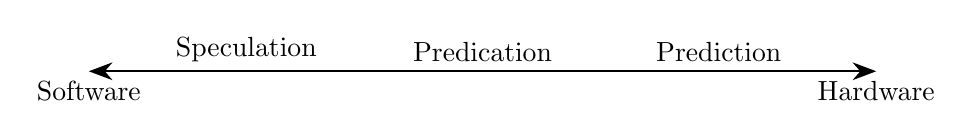
\begin{tikzpicture}[align=center]

\draw[arrows={Stealth[length=3mm]-Stealth[length=3mm]}, thick] (0,0) -- (10,0);

% Place labels at the ends
\node[below] at (0,0) {Software};
\node[below] at (10,0) {Hardware};

\node[above] at (2,0) {Speculation};
\node[above] at (5,0) {Predication};
\node[above] at (8,0) {Prediction};

\end{tikzpicture}
% \end{frame}

\begin{frame}{Compiler-Controlled Speculation}
\begin{itemize}
    \item During runtime, we only know the pipeline
    \item During compilation, we know the global picture
\end{itemize}
    \begin{block}{Speculative Execution}
        \begin{itemize}
            \item Make assumptions about future control flow
            \item \textbf{Execute before we know we need the result} 
            \item This includes moving instructions across branches
            \item \textbf{Risk:} May alter the program's execution \& result
        \end{itemize}
    \end{block}
\end{frame}

\begin{frame}{Restrictions for Speculation}
    \begin{center}
        \begin{minipage}{0.45\textwidth}
            \centering
            \begin{lstlisting}[style=AsmStyle]    
    LDR r1, [address]
    CMP r1, #0
    BEQ taken
    SDIV r1, #5, r1
    B end
taken:
    ADD r1, r1, #2
end:
\end{lstlisting}
        \end{minipage}
        \hfill
        \begin{minipage}{0.45\textwidth}
            \centering
            \begin{lstlisting}[style=AsmStyle]
    ldr r1, [address]
    ldr r2, [address2]
    @sdiv r2, #5, r1@
    beq taken, r1, #0
    b end
taken:
    add r1, r2, #2
end:
\end{lstlisting}
        \end{minipage}
    \end{center}
    \vspace{-0.9cm}
    \begin{center}
        \captionsetup{type=Listing}
        \captionof{lstlisting}{If we could schedule \texttt{sdiv} earlier, we likely increase ILP. However, it may overwrite \texttt{r2} used in \texttt{taken} or throw an exception}
        \label{fig:restrictions_speculation}
    \end{center}
        \vspace{-1cm}
        %If we want to move an instruction \texttt{I} above its control branch \texttt{Br}:
    \begin{block}{If we want to move an instruction I above its branch Br:}
        \begin{itemize}
            \item \textbf{Restriction 1}: The destination register of I is not used as a source if Br is taken
            \item \textbf{Restriction 2}: Instruction I will not cause an exception which will alter the program
execution if Br is taken.
        \end{itemize}
    \end{block}
\end{frame}

\begin{frame}{Computing the Average of Absolute Values}
    \begin{columns}[T]
        \begin{column}{0.53\textwidth}
            \begin{itemize}
                \item Go through all nodes
                \item If \texttt{wt} is negative, subtract it from \texttt{weight}
                \item Else, add it to \texttt{weight}
                \item Compute \texttt{avg} if we had at least one node
            \end{itemize}
        \end{column}

        \begin{column}{0.45\textwidth}
            \begin{minipage}{\textwidth}
                \begin{lstlisting}[style=CStyle]
avg = 0;
weight = 0;
count = 0;

while (ptr != NULL) {
	count++;
	if(ptr->wt < 0) {
		weight -= ptr->wt;
	} else {
		weight += ptr->wt;
	}
	ptr = ptr->next;
}

if(count !=0) {
	avg = weight / count;
}
\end{lstlisting}
                \label{ls:ls_c_chang_full_default}
            \end{minipage}
        \end{column}
    \end{columns}
\end{frame}

\begin{frame}{Steps}
        \begin{block}{Typical Ingredients}
        \begin{enumerate}
            \item Identify \textit{trace}
            \item Superblock creation
            \item Dependency graph (based on architectural model)
            \item List scheduling
        \end{enumerate}
    \end{block}
\end{frame}

\begin{frame}{Control Flow Profile}
    \begin{columns}[T]
        \begin{column}{0.47\textwidth}
            \begin{block}{Profiling}
                \begin{itemize}
                    \item Collect execution data
                    \item Facilitate optimization decisions
                    \item E.g. in LLVM~\cite{llvm_profdata} with \texttt{-fprofile-instr-generate}
                \end{itemize}
            \end{block}
            \begin{itemize}
                \item The loop part BB2 to BB5 is interesting
                \item 90\% of the weights are positive
            \end{itemize}
        \end{column}

        \begin{column}{0.53\textwidth}
            \centering
            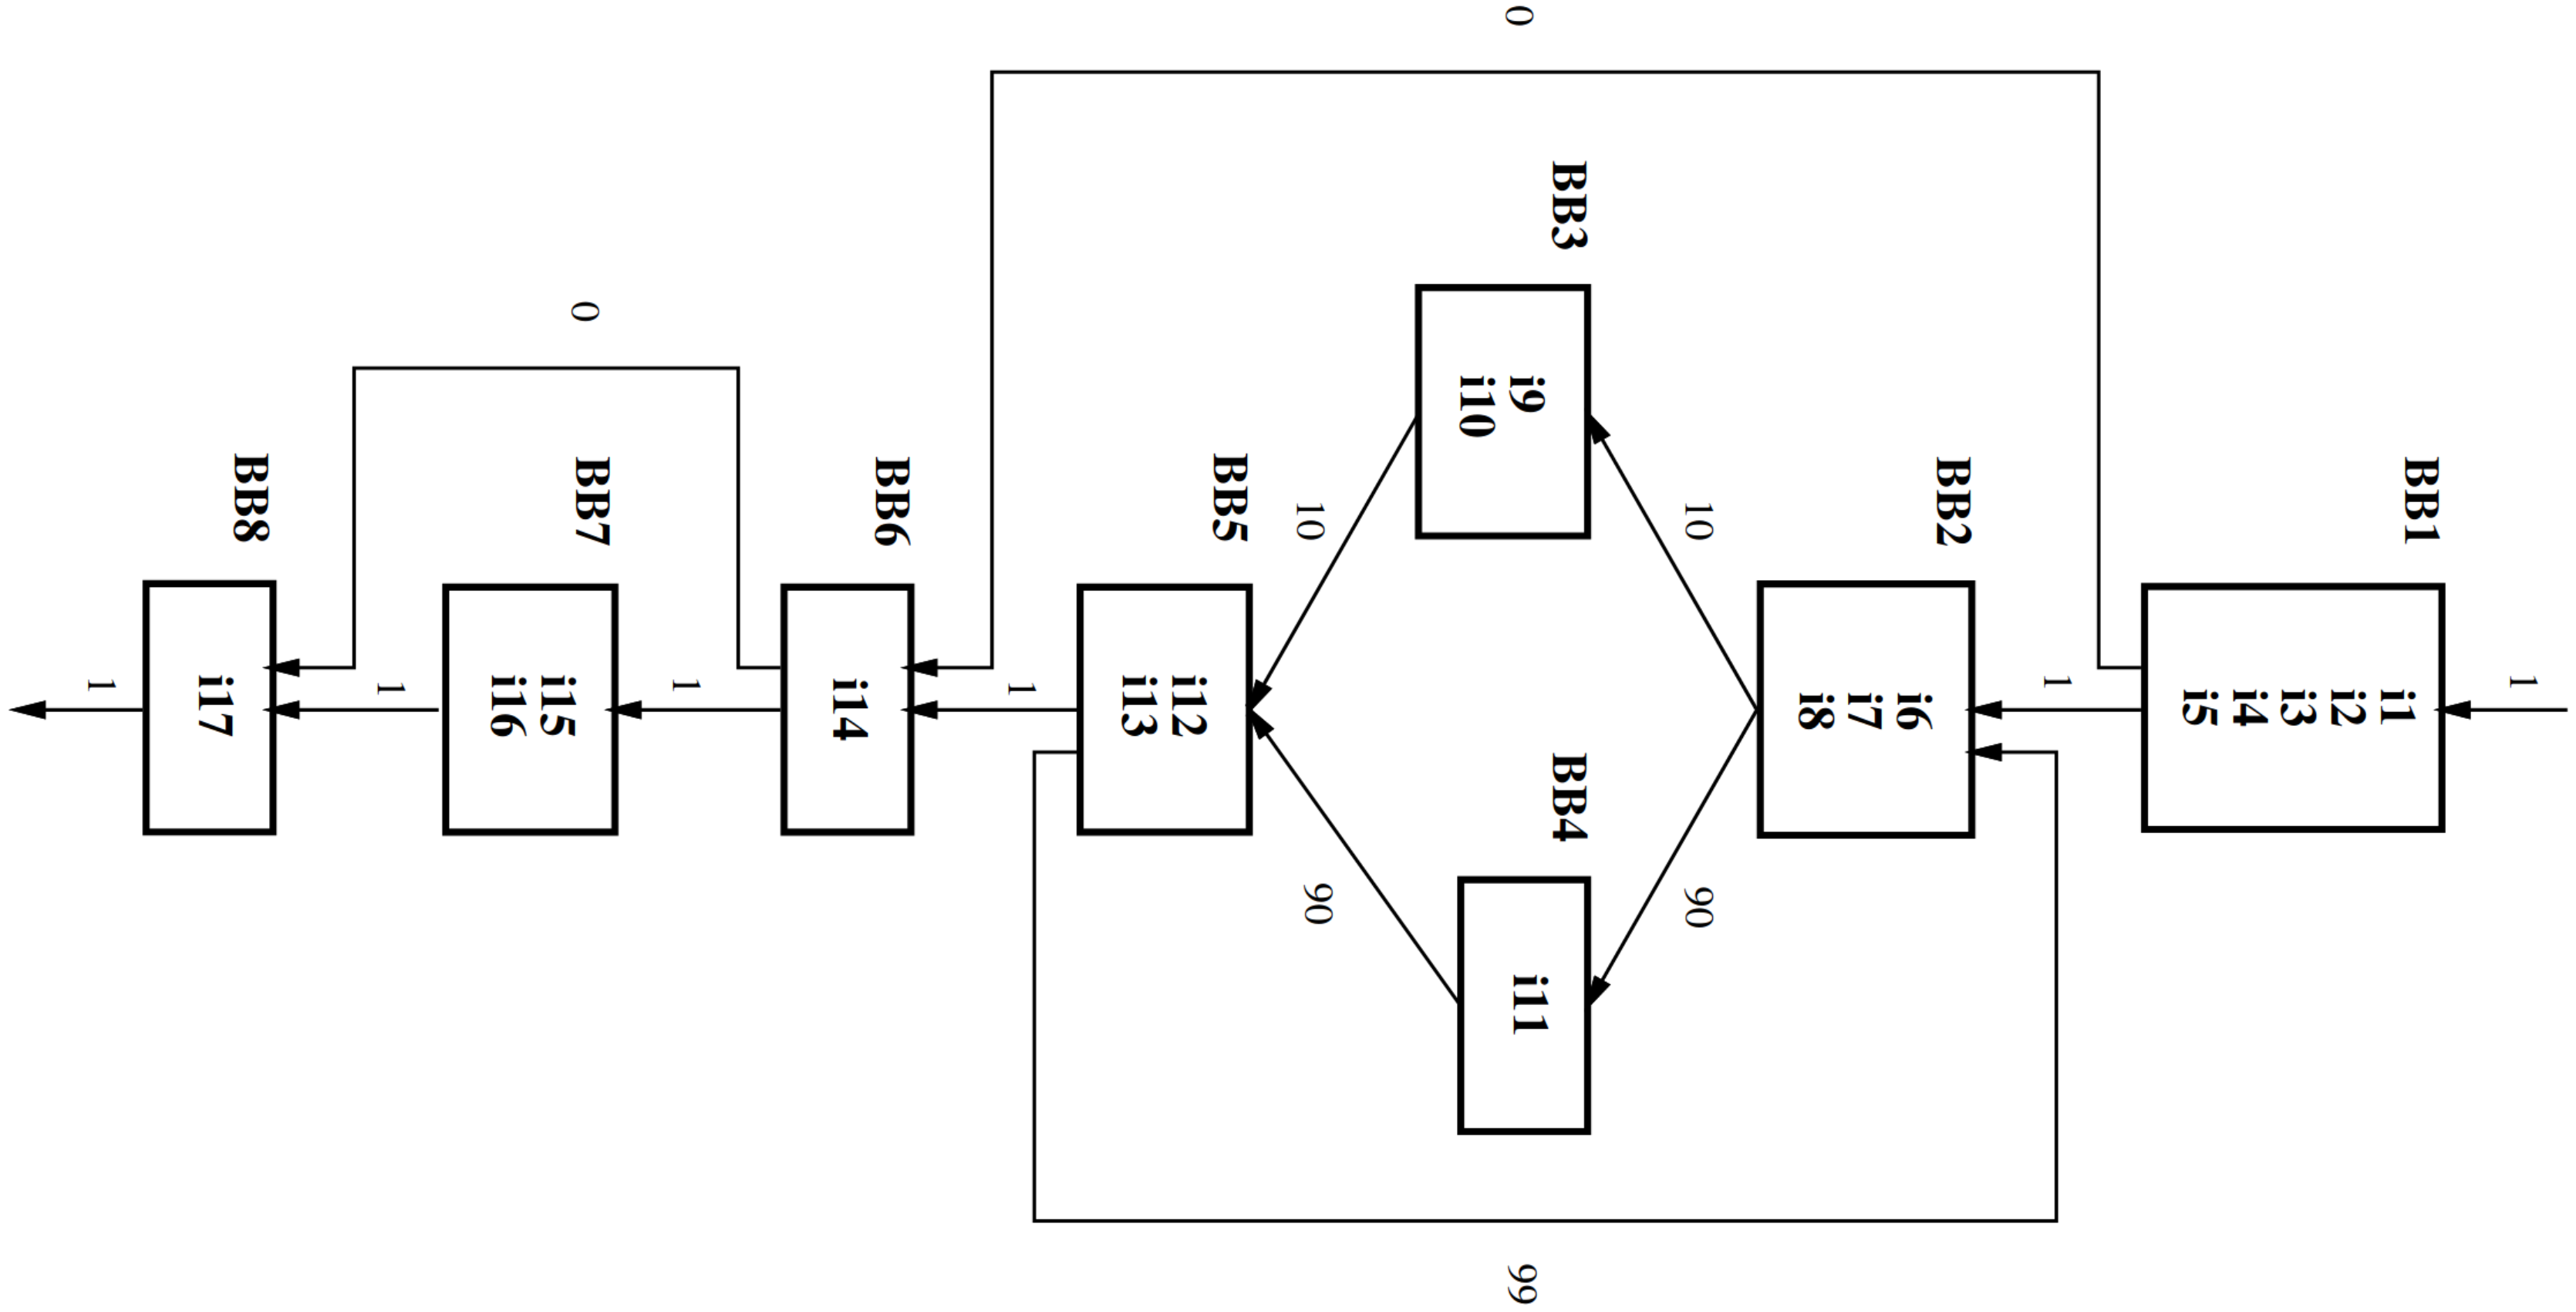
\includegraphics[width=1\linewidth, angle=90]{src//figure//image/image_chang_default_cfg.png}
            \captionof{figure}{Weighted Control Flow Graph with profiling data of Chang~\cite{chang95}}
            \label{fig:controlflow_full}
        \end{column}
    \end{columns}
\end{frame}

\begin{frame}{Loop Part as a Superblock}
    \begin{minipage}{0.89\textwidth}
        \centering
        \begin{minipage}{0.38\textwidth}
            \centering
            \resizebox{\textwidth}{!}{%
                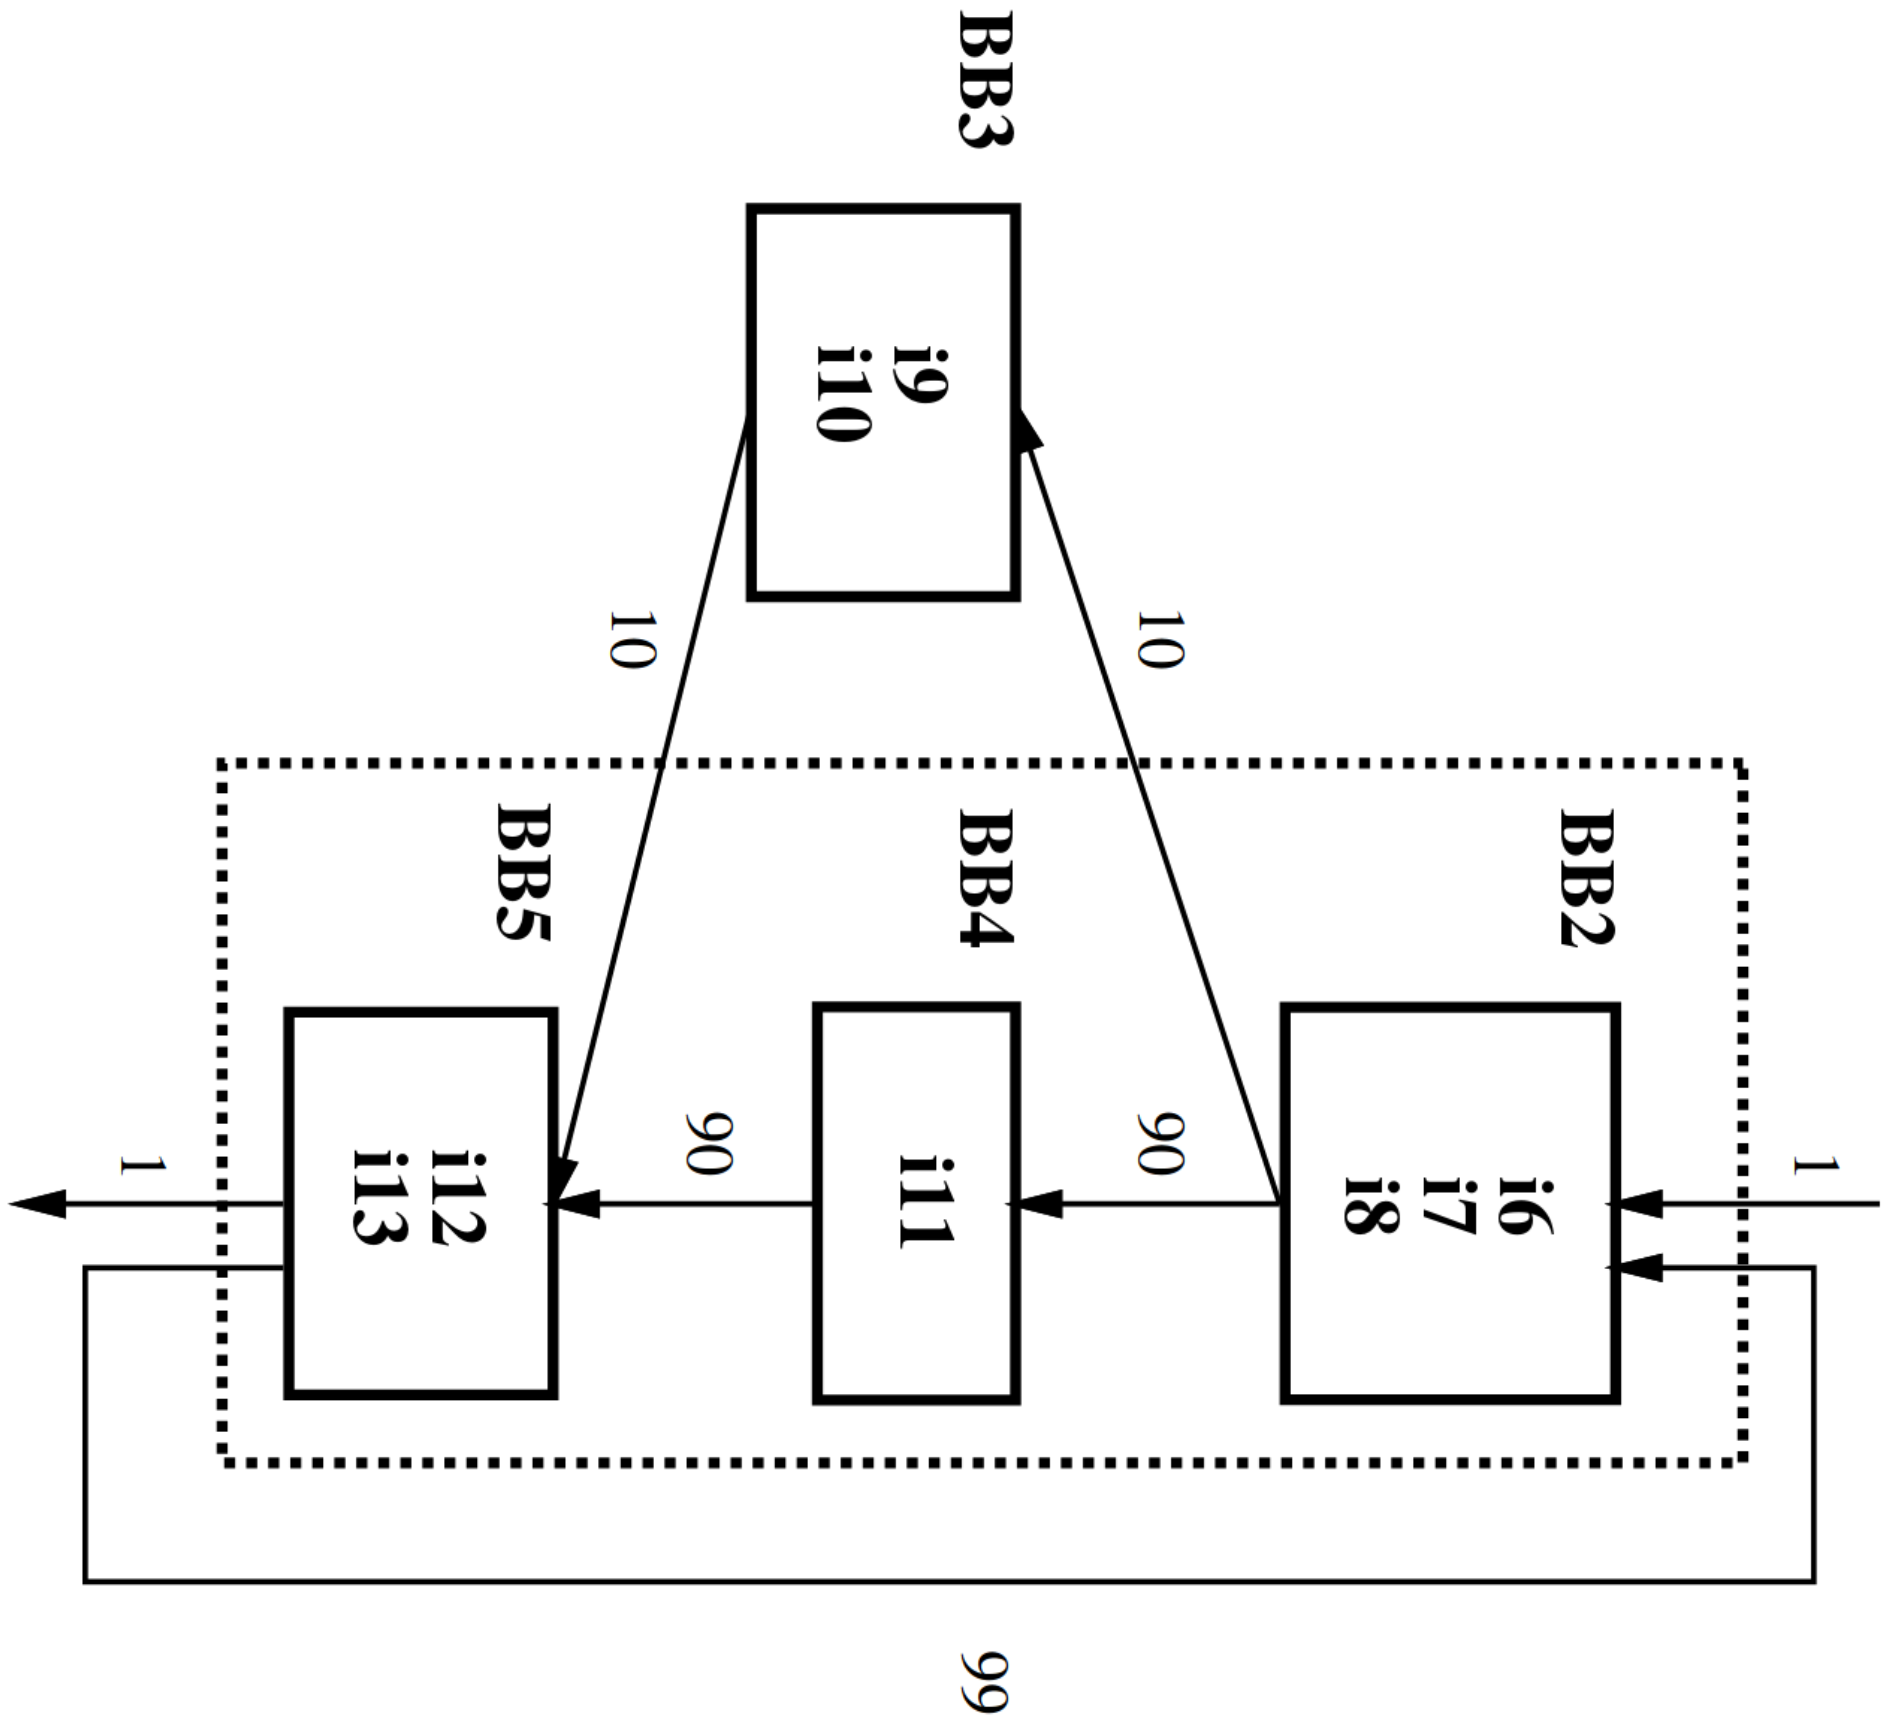
\includegraphics[width=\linewidth, angle=90]{src//figure//image/image_chang_loop_cfg.png}

            }
            \label{fig:controlflow_side_enterance}
        \end{minipage}\hfill
        \begin{minipage}{0.58\textwidth}
            \centering
            \resizebox{\textwidth}{!}{%
                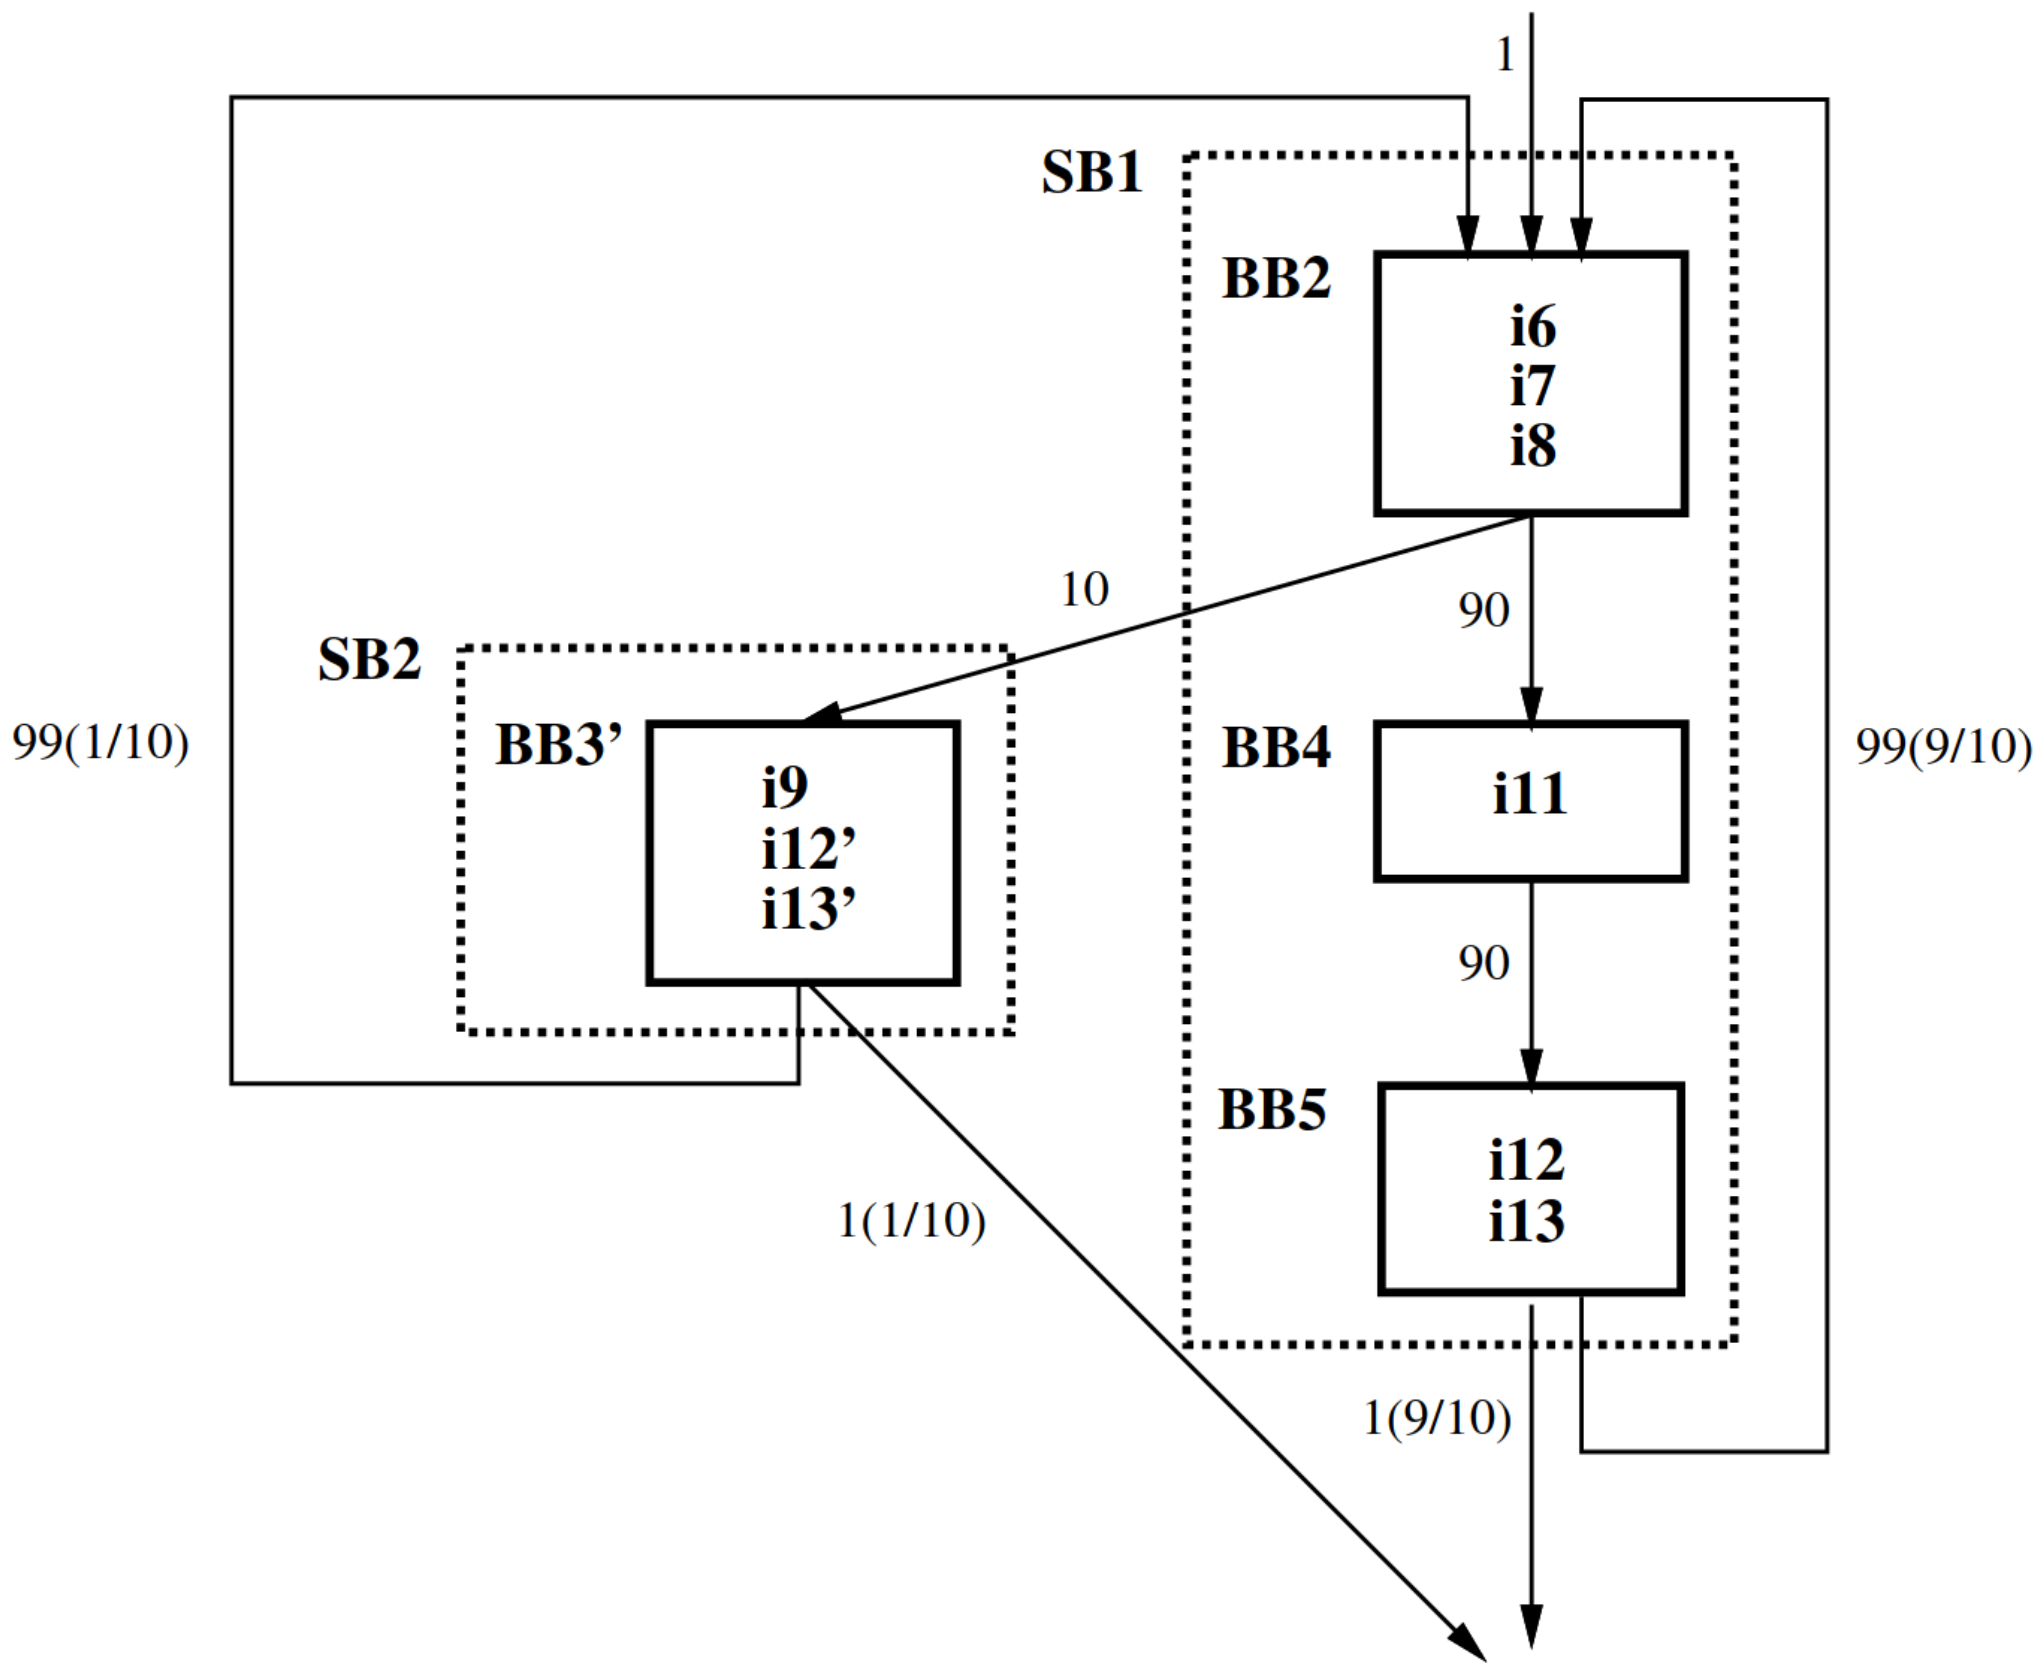
\includegraphics[width=0.5\linewidth]{src//figure//image/image_chang_sb_loop_cfg.png}

            }
            \label{fig:controlflow_superblock}
        \end{minipage}
    \end{minipage}

    \vspace{-0.7cm}
    \begin{minipage}{\textwidth}
        \centering
        \captionof{figure}{Loop before and after Superblock creation~\cite{chang95}. BB5 is duplicated in BB3'}
    \end{minipage}

    \begin{minipage}{\textwidth}
        \begin{block}{BB2 $\rightarrow$ BB4 $\rightarrow$ BB5 is the hot part (\textit{trace})}
            \begin{itemize}
                \item Superblocks reduce bookkeeping~\cite{sb_art}
                \item No need to consider side entrances when scheduling a superblock
            \end{itemize}
        \end{block}
    \end{minipage}
\end{frame}


\begin{frame}{Models for Speculative Scheduling}
    \begin{block}{Different Code Percolation Models}
        \begin{itemize}
            \item Enable different levels of speculation
            \item And hence different levels of performance
            \item Can alter the result of the program
            \item Require additional hardware
        \end{itemize}
    \end{block}
    \vspace{0.9cm}
        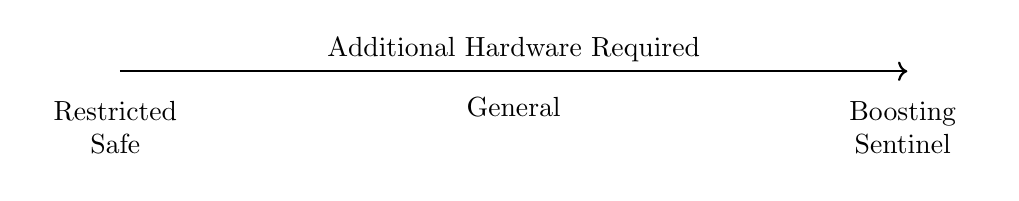
\begin{tikzpicture}[align=center, node distance=0cm and 1cm]

    \draw[->, thick] (0,0) -- (10,0);
    \node[above=0cm] at (5,0) {Additional Hardware Required};
    \node[below=0.2cm] at (0,0) {
        \begin{tabular}{c}
            Restricted \\
            Safe
        \end{tabular}
    };
    \node[below=0.2cm] at (5,0) {General};
    \node[below=0.2cm] at (10,0) {
        \begin{tabular}{c}
            Boosting \\
            Sentinel
        \end{tabular}
    };

\end{tikzpicture}

\end{frame}

\begin{frame}{Scheduling our Superblock (Report page 22)}
    \begin{center}
    \begin{minipage}{1\textwidth}
        \begin{center}
                \resizebox{0.57\textwidth}{!}{
                    \begin{minipage}{\textwidth}
                        \begin{lstlisting}[style=AsmStyle]
    ldr r1, _ptr      ; Initialize
    mov r7, 0         
    mov r2, 0         
    mov r3, 0         
    beq L3, r1, 0     
L0:
    add r2, r2, 1     ; I1: Increment count
    ldr r4, 0[r1]     ; I2: Load ptr->wt into r4
    btl L1, r4, 0     ; I3: If wt < 0, branch to L1
    add r3, r3, r4    ; I4: Add wt to weight
    ldr r5, 4[r1]     ; I5: Load ptr->next into r5
    beq L3, r5, 0     ; I6: If next is NULL, jump to L3
    add r2, r2, 1     ; I7: Increment count
    ldr r6, 0[r5]     ; I8: Load next->wt into r6
    btl L1X, r6, 0    ; I9: If wt < 0, branch to L1X
    add r3, r3, r6    ; I10: Add wt to weight
    ldr r1, 4[r5]     ; I11: Move ptr to ptr->next->next
    bne L0, r1, 0     ; I12: Loop back to L0 if ptr != NULL
L3:
    beq L4, r2, 0     ; If count == 0, skip division
    div r7, r3, r2    
    str _avg, r7      
L4:
; ...
L1X:
    mov r1, r5        ; Adjust ptr = ptr->next
    mov r4, r6        ; Move wt to r4 for subtraction
L1: 
    sub r3, r3, r4    ; Subtract wt from weight
    ldr r1, 4[r1]     ; Move ptr to ptr->next
    bne L0, r1, 0     ; Loop back to L0 if ptr != NULL
\end{lstlisting}

                    \end{minipage}
                }
        
        \vspace{-0.2cm}
        \captionsetup{type=Listing}
        \captionof{lstlisting}{The loop part of the superblock was unrolled once. We assume a one-cycle latency for ALU instructions and a two-cycle load delay.}
        \end{center}
        \end{minipage}
    \end{center}
\end{frame}

%%% Restricted %%%
\begin{frame}{Restricted Code Percolation}
    \begin{block}{Properties of Restricted Code Percolation}
        \begin{itemize}
            \item \textit{Avoid errors} category~\cite{bringmannMH95}
            \item Compiler cannot move excepting instructions above branches
            \item Other instructions which fulfill Restriction 1 can be moved
                \begin{itemize}
                    \item E.g. after renaming
                \end{itemize}
            \item Requires no additional hardware
            \item No extra load on DCache
        \end{itemize}
    \end{block}
    \begin{block}{Safe Code Percolation Extension~\cite{bringmannMH95}}
        \begin{itemize}
            \item Restriction 2 can be relaxed 
            \begin{itemize}
                \item If there is a proof that the instructions will never cause an exception
            \end{itemize}     
            \item Typically speculative loads by check allocation boundaries
        \end{itemize}
    \end{block}
\end{frame}

\begin{frame}{Restricted Code Percolation}
    \begin{center}
    \begin{minipage}{.52\textwidth}
        \begin{figure}[H]
            \centering
            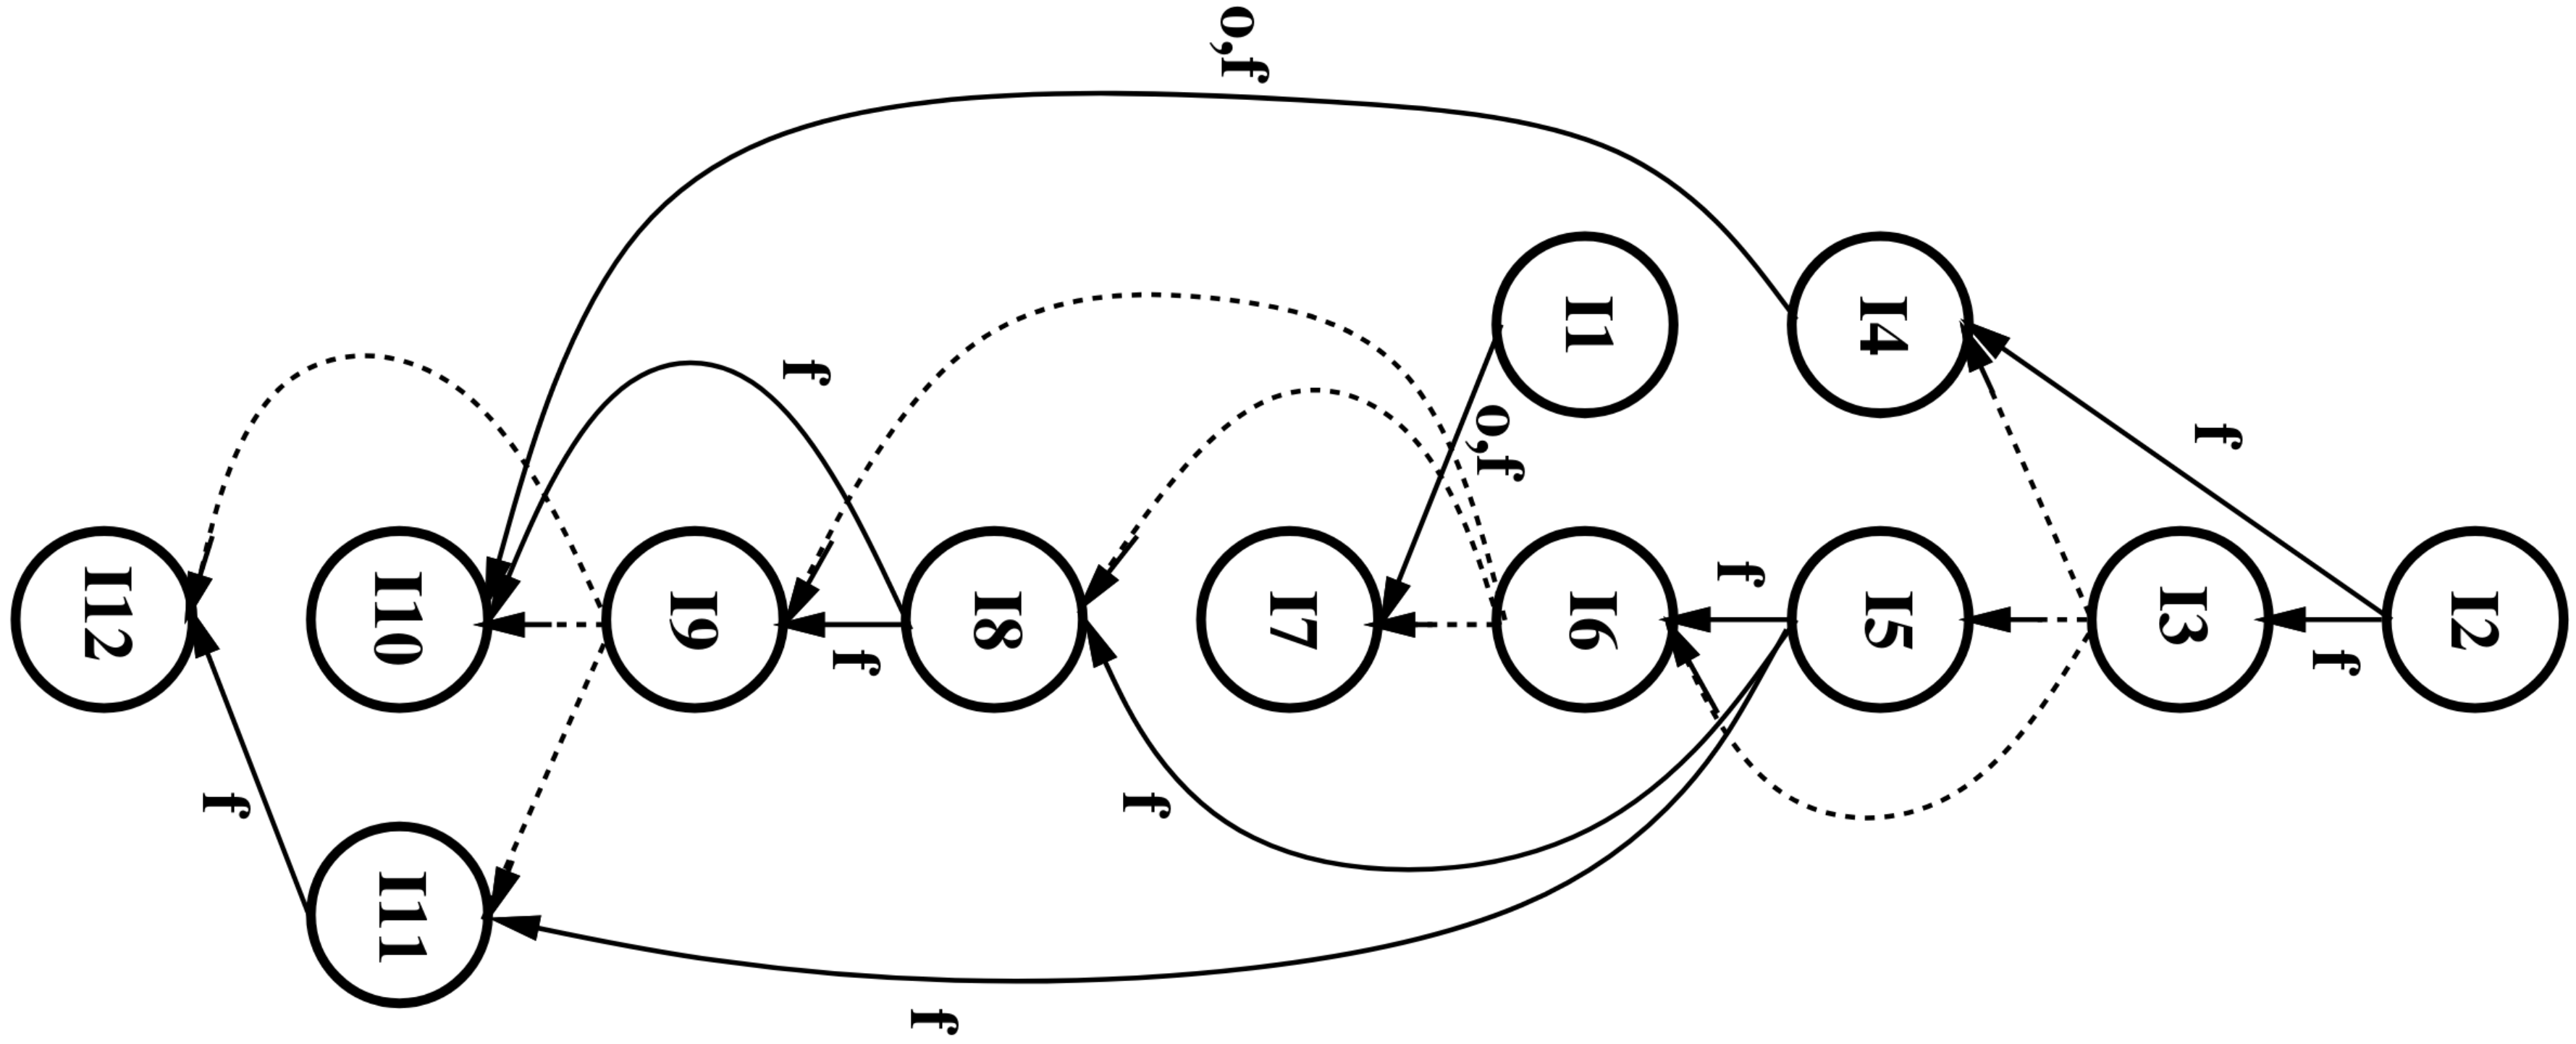
\includegraphics[width=\linewidth, angle=90]{src/figure/image/restricted_cfg.png}

            \caption{Nine dashed control dependencies and twelve data dependencies (\textbf{f}low, \textbf{o}utput) under restricted percolation~\cite{chang95}.}
            \label{fig:restric_cfg}
\end{figure}
    \end{minipage}\hfill
    \begin{minipage}{.46\textwidth}
    \begin{figure}[H]
            \centering
            \resizebox{1\textwidth}{!}{
            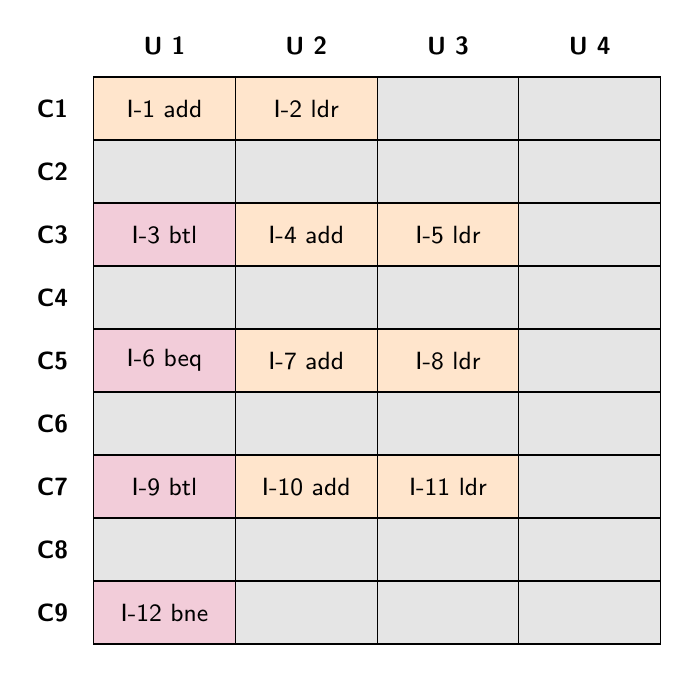
\begin{tikzpicture}[font=\sffamily, scale=1]
\def\cellwidth{1.8}
\def\cellheight{0.8}

\newlength{\cellwidthLength}
\setlength{\cellwidthLength}{\cellwidth cm}
\newlength{\cellheightLength}
\setlength{\cellheightLength}{\cellheight cm}

\tikzstyle{ALU} = [fill=orange!20, draw=black, rectangle, minimum width=\cellwidthLength, minimum height=\cellheightLength]
\tikzstyle{LOAD} = [fill=orange!20, draw=black, rectangle, minimum width=\cellwidthLength, minimum height=\cellheightLength]
\tikzstyle{BRANCH} = [fill=purple!20, draw=black, rectangle, minimum width=\cellwidthLength, minimum height=\cellheightLength]
\tikzstyle{EMPTY} = [fill=gray!20, draw=black, rectangle, minimum width=\cellwidthLength, minimum height=\cellheightLength]

\def\numcycles{9}
\def\numunits{4}

\foreach \i in {1,...,\numcycles} {
    \foreach \j in {1,...,\numunits} {
        \pgfmathsetmacro{\x}{(\j - 1) * \cellwidth}
        \pgfmathsetmacro{\y}{-\i * \cellheight}
        \draw[EMPTY] (\x cm, \y cm) rectangle ++(\cellwidthLength, \cellheightLength);
    }
}

\foreach \j in {1,...,\numunits} {
    \pgfmathsetmacro{\x}{(\j - 1) * \cellwidth + 0.5 * \cellwidth}
    \node at (\x cm, 0.5 * \cellheight cm) {\small\textbf{U \j}};
}

\foreach \i in {1,...,\numcycles} {
    \pgfmathsetmacro{\y}{-\i * \cellheight + 0.5 * \cellheight}
    \node[anchor=east] at (-0.2 cm, \y cm) {\small\textbf{C\i}};
}


% Cycle 1
\pgfmathsetmacro{\y}{-1 * \cellheight}
\draw[ALU] (0 cm, \y cm) rectangle ++(\cellwidthLength, \cellheightLength) node[pos=.5] {\small I-1 add};
\draw[LOAD] (\cellwidth cm, \y cm) rectangle ++(\cellwidthLength, \cellheightLength) node[pos=.5] {\small I-2 ldr};

% Cycle 3
\pgfmathsetmacro{\y}{-3 * \cellheight}
\draw[BRANCH] (0 cm, \y cm) rectangle ++(\cellwidthLength, \cellheightLength) node[pos=.5] {\small I-3 btl};
\draw[ALU] (\cellwidth cm, \y cm) rectangle ++(\cellwidthLength, \cellheightLength) node[pos=.5] {\small I-4 add};
\draw[LOAD] (2 * \cellwidth cm, \y cm) rectangle ++(\cellwidthLength, \cellheightLength) node[pos=.5] {\small I-5 ldr};

% Cycle 5
\pgfmathsetmacro{\y}{-5 * \cellheight}
\draw[BRANCH] (0 cm, \y cm) rectangle ++(\cellwidthLength, \cellheightLength) node[pos=.5] {\small I-6 beq};
\draw[ALU] (\cellwidth cm, \y cm) rectangle ++(\cellwidthLength, \cellheightLength) node[pos=.5] {\small I-7 add};
\draw[LOAD] (2 *\cellwidth cm, \y cm) rectangle ++(\cellwidthLength, \cellheightLength) node[pos=.5] {\small I-8 ldr};

% Cycle 7
\pgfmathsetmacro{\y}{-7 * \cellheight}
\draw[BRANCH] (0 cm, \y cm) rectangle ++(\cellwidthLength, \cellheightLength) node[pos=.5] {\small I-9 btl};
\draw[ALU] (\cellwidth cm, \y cm) rectangle ++(\cellwidthLength, \cellheightLength) node[pos=.5] {\small I-10 add};
\draw[LOAD] (2 * \cellwidth cm, \y cm) rectangle ++(\cellwidthLength, \cellheightLength) node[pos=.5] {\small I-11 ldr};

% Cycle 9
\pgfmathsetmacro{\y}{-9 * \cellheight}
\draw[BRANCH] (0 cm, \y cm) rectangle ++(\cellwidthLength, \cellheightLength) node[pos=.5] {\small I-12 bne};

\foreach \i in {1,...,\numcycles} {
    \foreach \j in {1,...,\numunits} {
        \pgfmathsetmacro{\x}{(\j - 1) * \cellwidth}
        \pgfmathsetmacro{\y}{-\i * \cellheight}
        \draw (\x cm, \y cm) rectangle ++(\cellwidthLength, \cellheightLength);
    }
}

\end{tikzpicture} 
        }
        \caption{The schedule tableau is quite sparse. Loads have to stay in their home block. After \texttt{C1}, all data dependencies for \texttt{I7} are available.}
        \label{fig:restricted_motion}
\end{figure}
    \end{minipage}
\end{center} 
\end{frame}

\begin{frame}{But \texttt{I7}'s destination \texttt{r2} is in \texttt{live-out(I6)}}
    
\begin{center}
        \resizebox{0.62\textwidth}{!}{
            \begin{minipage}{\textwidth}
                \begin{lstlisting}[style=AsmStyle]
    ldr r1, _ptr      ; Initialize
    mov r7, 0         
    mov r2, 0         
    mov r3, 0         
    beq L3, r1, 0     
L0:
    add r2, r2, 1     ; I1: Increment count
    ldr r4, 0[r1]     ; I2: Load ptr->wt into r4
    btl L1, r4, 0     ; I3: If wt < 0, branch to L1
    add r3, r3, r4    ; I4: Add wt to weight
    ldr r5, 4[r1]     ; I5: Load ptr->next into r5
    @@beq L3, r5, 0     ; I6: If next is NULL, jump to L3
    @add r2, r2, 1     ; I7: Increment count
    ldr r6, 0[r5]     ; I8: Load next->wt into r6
    btl L1X, r6, 0    ; I9: If wt < 0, branch to L1X
    add r3, r3, r6    ; I10: Add wt to weight
    ldr r1, 4[r5]     ; I11: Move ptr to ptr->next->next
    bne L0, r1, 0     ; I12: Loop back to L0 if ptr != NULL
L3:
    @@beq L4, r2, 0     ; If count == 0, skip division
    @@div r7, r3, r2
    str _avg, r7      
L4:
; ...
L1X:
    mov r1, r5        ; Adjust ptr = ptr->next
    mov r4, r6        ; Move wt to r4 for subtraction
L1: 
    sub r3, r3, r4    ; Subtract wt from weight
    ldr r1, 4[r1]     ; Move ptr to ptr->next
    bne L0, r1, 0     ; Loop back to L0 if ptr != NULL
\end{lstlisting}

            \end{minipage}
        }
\end{center}
\end{frame}
%%% %%% %%%


%%% General %%%
\begin{frame}{General Code Percolation}
    \begin{block}{Properties of General Code Percolation}
        \begin{itemize}
            \item \textit{Ignore errors} category
            \item Lifts Restriction 2 by simply ignoring exceptions
            \item Requires non-excepting counterpart instructions
        \end{itemize}
    \end{block}
    \begin{itemize}
        \item E.g., if a load accesses an invalid address, its destination will be garbage
        \item May cause an actual exception later if the result is used
    \end{itemize}
\end{frame}

\begin{frame}{General Code Percolation}
    \begin{center}
    \begin{minipage}{.52\textwidth}
        \begin{figure}[H]
            \centering
            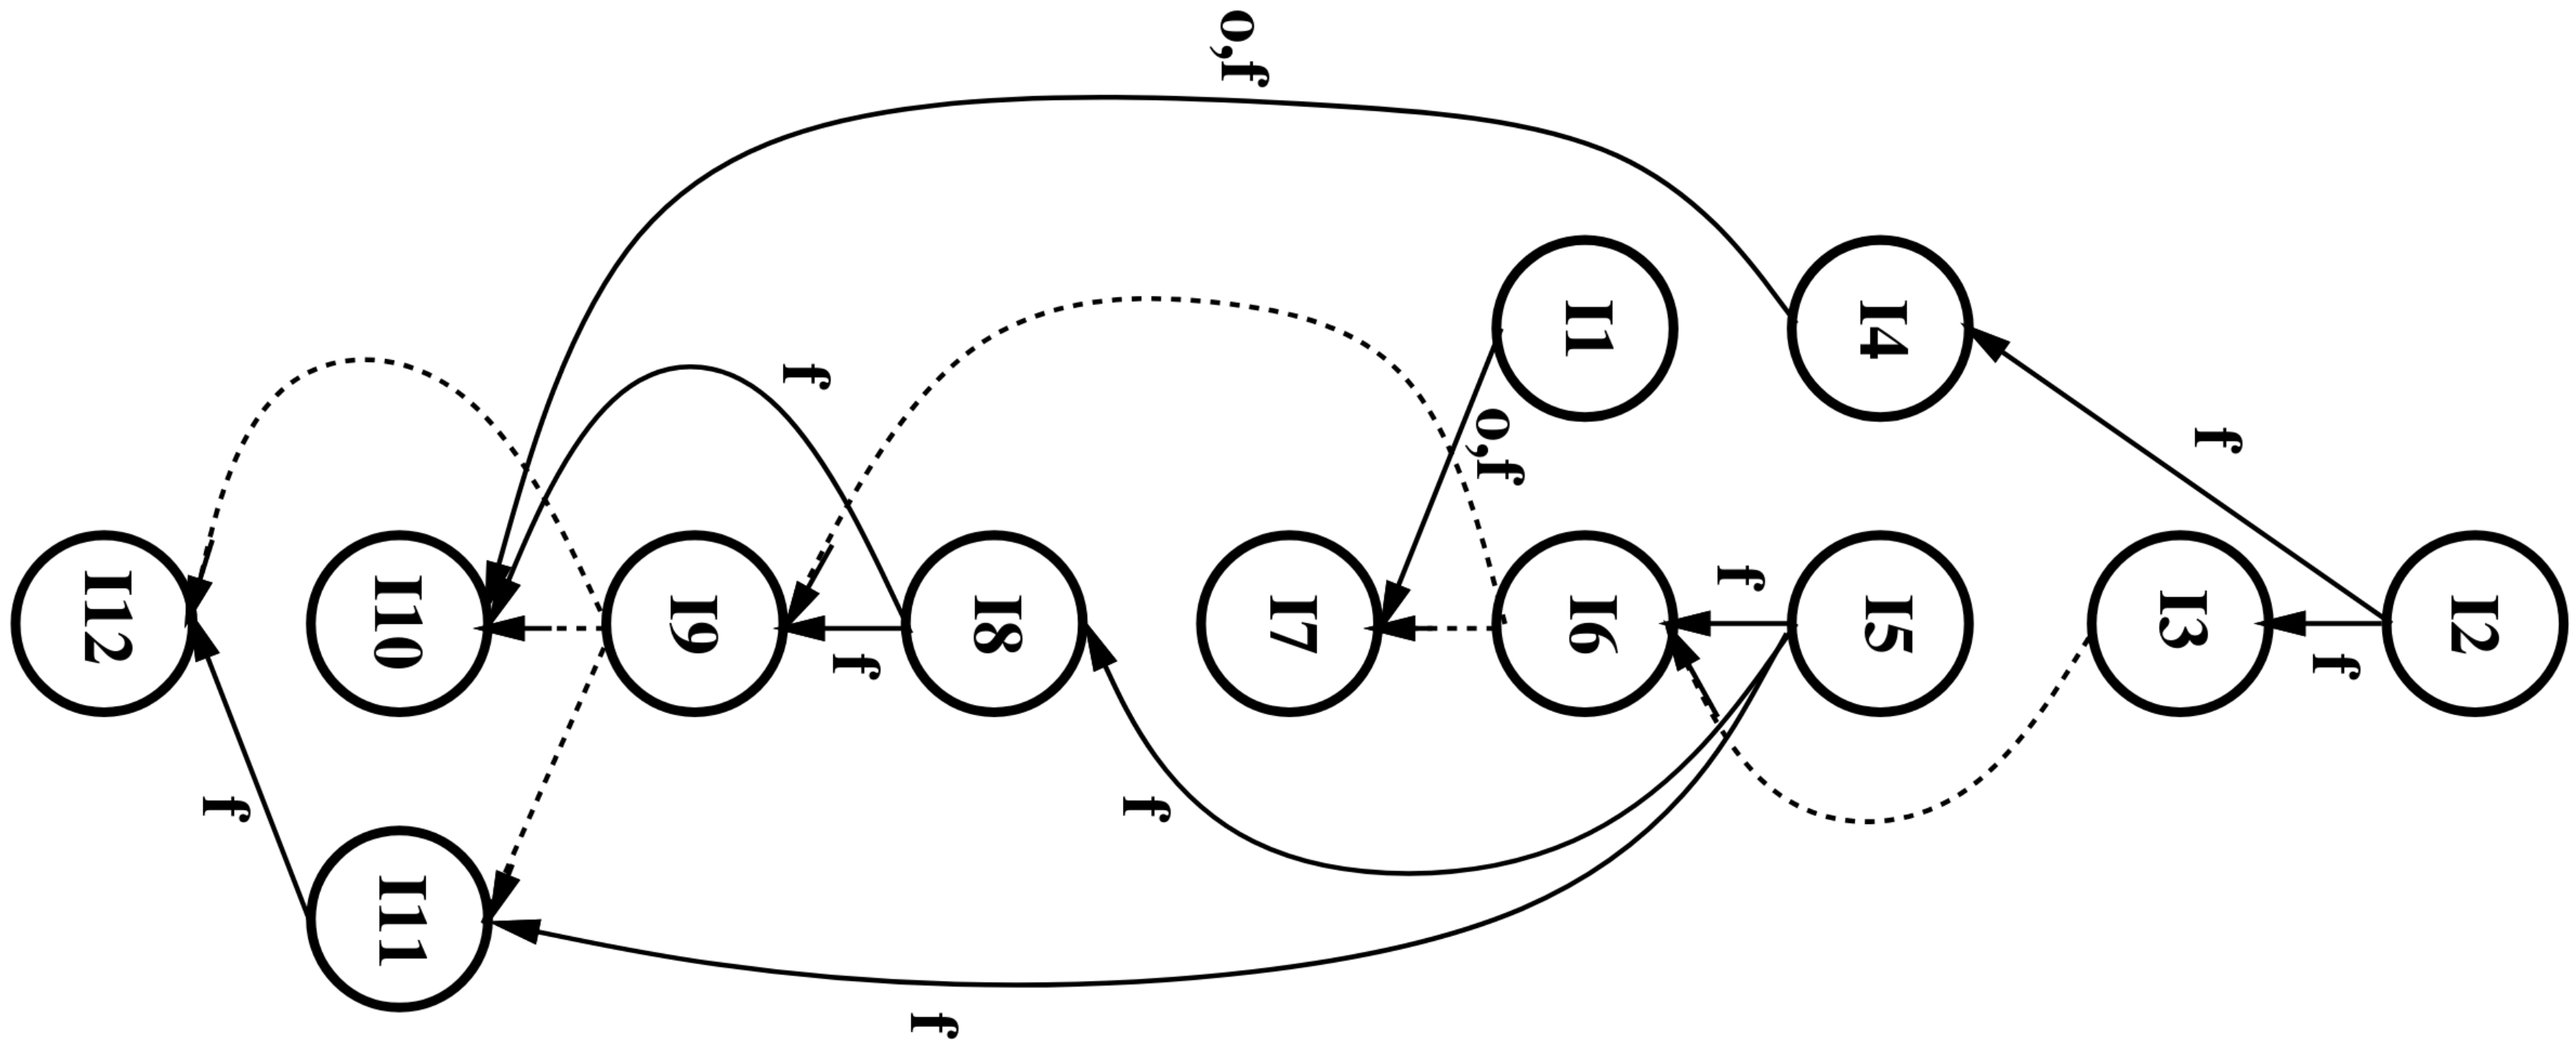
\includegraphics[width=\linewidth, angle=90]{src/figure/image/general_cfg.png}

            \caption{Dependence Graph for General Code Percolation with six control dependencies~\cite{chang95}.}
\end{figure}
    \end{minipage}\hfill
    \begin{minipage}{.46\textwidth}
\begin{figure}[H]
            \centering
            \resizebox{1\textwidth}{!}{
            \begin{tikzpicture}[font=\sffamily, scale=1]
\def\cellwidth{1.8}
\def\cellheight{0.8}

% Define lengths with units
%\newlength{\cellwidthLength}
\setlength{\cellwidthLength}{\cellwidth cm}
%\newlength{\cellheightLength}
\setlength{\cellheightLength}{\cellheight cm}

\tikzstyle{ALU} = [fill=orange!20, draw=black, rectangle, minimum width=\cellwidthLength, minimum height=\cellheightLength]
\tikzstyle{LOAD} = [fill=orange!20, draw=black, rectangle, minimum width=\cellwidthLength, minimum height=\cellheightLength]
\tikzstyle{BRANCH} = [fill=purple!20, draw=black, rectangle, minimum width=\cellwidthLength, minimum height=\cellheightLength]
\tikzstyle{EMPTY} = [fill=gray!20, draw=black, rectangle, minimum width=\cellwidthLength, minimum height=\cellheightLength]

\def\numcycles{5}
\def\numunits{4}

\foreach \i in {1,...,\numcycles} {
    \foreach \j in {1,...,\numunits} {
        \pgfmathsetmacro{\x}{(\j - 1) * \cellwidth}
        \pgfmathsetmacro{\y}{-\i * \cellheight}
        \draw[EMPTY] (\x cm, \y cm) rectangle ++(\cellwidthLength, \cellheightLength);
    }
}

\foreach \j in {1,...,\numunits} {
    \pgfmathsetmacro{\x}{(\j - 1) * \cellwidth + 0.5 * \cellwidth}
    \node at (\x cm, 0.5 * \cellheight cm) {\small\textbf{U \j}};
}

\foreach \i in {1,...,\numcycles} {
    \pgfmathsetmacro{\y}{-\i * \cellheight + 0.5 * \cellheight}
    \node[anchor=east] at (-0.2 cm, \y cm) {\small\textbf{C\i}};
}

% Cycle 1
\pgfmathsetmacro{\y}{-1 * \cellheight}
\draw[ALU] (0 cm, \y cm) rectangle ++(\cellwidthLength, \cellheightLength) node[pos=.5] {\small I-1 add};
\draw[LOAD] (\cellwidth cm, \y cm) rectangle ++(\cellwidthLength, \cellheightLength) node[pos=.5] {\small I-2 ldr};
\draw[LOAD] (2 * \cellwidth cm, \y cm) rectangle ++(\cellwidthLength, \cellheightLength) node[pos=.5] {\small I-5 ldr};

% Cycle 3
\pgfmathsetmacro{\y}{-3 * \cellheight}
\draw[BRANCH] (0 cm, \y cm) rectangle ++(\cellwidthLength, \cellheightLength) node[pos=.5] {\small I-3 btl};
\draw[ALU] (\cellwidth cm, \y cm) rectangle ++(\cellwidthLength, \cellheightLength) node[pos=.5] {\small I-4 add};
\draw[LOAD] (2 * \cellwidth cm, \y cm) rectangle ++(\cellwidthLength, \cellheightLength) node[pos=.5] {\small I-8 ldr};
\draw[LOAD] (3 * \cellwidth cm, \y cm) rectangle ++(\cellwidthLength, \cellheightLength) node[pos=.5] {\small I-11 ldr};

% Cycle 4
\pgfmathsetmacro{\y}{-4 * \cellheight}
\draw[BRANCH] (0 cm, \y cm) rectangle ++(\cellwidthLength, \cellheightLength) node[pos=.5] {\small I-6 beq};

% Cycle 5
\pgfmathsetmacro{\y}{-5 * \cellheight}
\draw[ALU] (0 cm, \y cm) rectangle ++(\cellwidthLength, \cellheightLength) node[pos=.5] {\small I-7 add};
\draw[BRANCH] (\cellwidth cm, \y cm) rectangle ++(\cellwidthLength, \cellheightLength) node[pos=.5] {\small I-9 btl};
\draw[ALU] (2 *\cellwidth cm, \y cm) rectangle ++(\cellwidthLength, \cellheightLength) node[pos=.5] {\small I-10 add};
\draw[BRANCH] (3 *\cellwidth cm, \y cm) rectangle ++(\cellwidthLength, \cellheightLength) node[pos=.5] {\small I-12 bne};

\foreach \i in {1,...,\numcycles} {
    \foreach \j in {1,...,\numunits} {
        \pgfmathsetmacro{\x}{(\j - 1) * \cellwidth}
        \pgfmathsetmacro{\y}{-\i * \cellheight}
        \draw (\x cm, \y cm) rectangle ++(\cellwidthLength, \cellheightLength);
    }
}

\end{tikzpicture} 
        }
        \caption{By lifting Restriction 2, we are able to schedule the loads earlier at the cost of eventual errors. E.g., \texttt{I8} which is now above \texttt{I6} (\texttt{next == null}) will cause errors.}
\end{figure}
    \end{minipage}
\end{center} 
\end{frame}
%%% %%% %%%

%%% Boosting %%%
\begin{frame}{Boosting Code Percolation}
    \begin{block}{Properties of Boosting Code Percolation}
        \begin{itemize}
            \item \textit{Resolve errors}
            \item Lifts Restriction 1 \& 2 with additional hardware support
            \item Temporarily hold side effects of a boosted instruction
            \begin{itemize}
                \item Until its branch is executed 
            \end{itemize}
        \end{itemize}
    \end{block}
\end{frame}

\begin{frame}{Hardware for Boosting}
   \begin{itemize}
       \item Superblock $\rightarrow$ Boosted instruction is in the not-taken part 
       \item 1 to N bits $\rightarrow$ above how many branches the instruction was moved
       \item Not taken while boosted instructions are in the pipeline $\rightarrow$ remove bit
       \item Taken while boosted instructions are in the pipeline $\rightarrow$ squash them
   \end{itemize} 
    \begin{block}{Shadow Register File \& Shadow Store Buffer~\cite{10.1145/325164.325160}}
        \begin{itemize}
       \item If boosted instruction writes back before its branch $\rightarrow$ keep its result
       \begin{itemize}
           \item And delay exception handling until we know the branch outcome
       \end{itemize}
       \item If branch is not taken $\rightarrow$ copy result into real register or store buffer
       \begin{itemize}
           \item If there was an exception, re-execute not-taken part in-order
       \end{itemize}
       \item If branch is taken $\rightarrow$ squash shadow values, ignore exceptions and go to branch target
   \end{itemize} 
    \end{block}
\end{frame}


\begin{frame}{Boosting Code Percolation}
    \begin{center}
    \begin{minipage}{.52\textwidth}
        \begin{figure}[H]
            \centering
            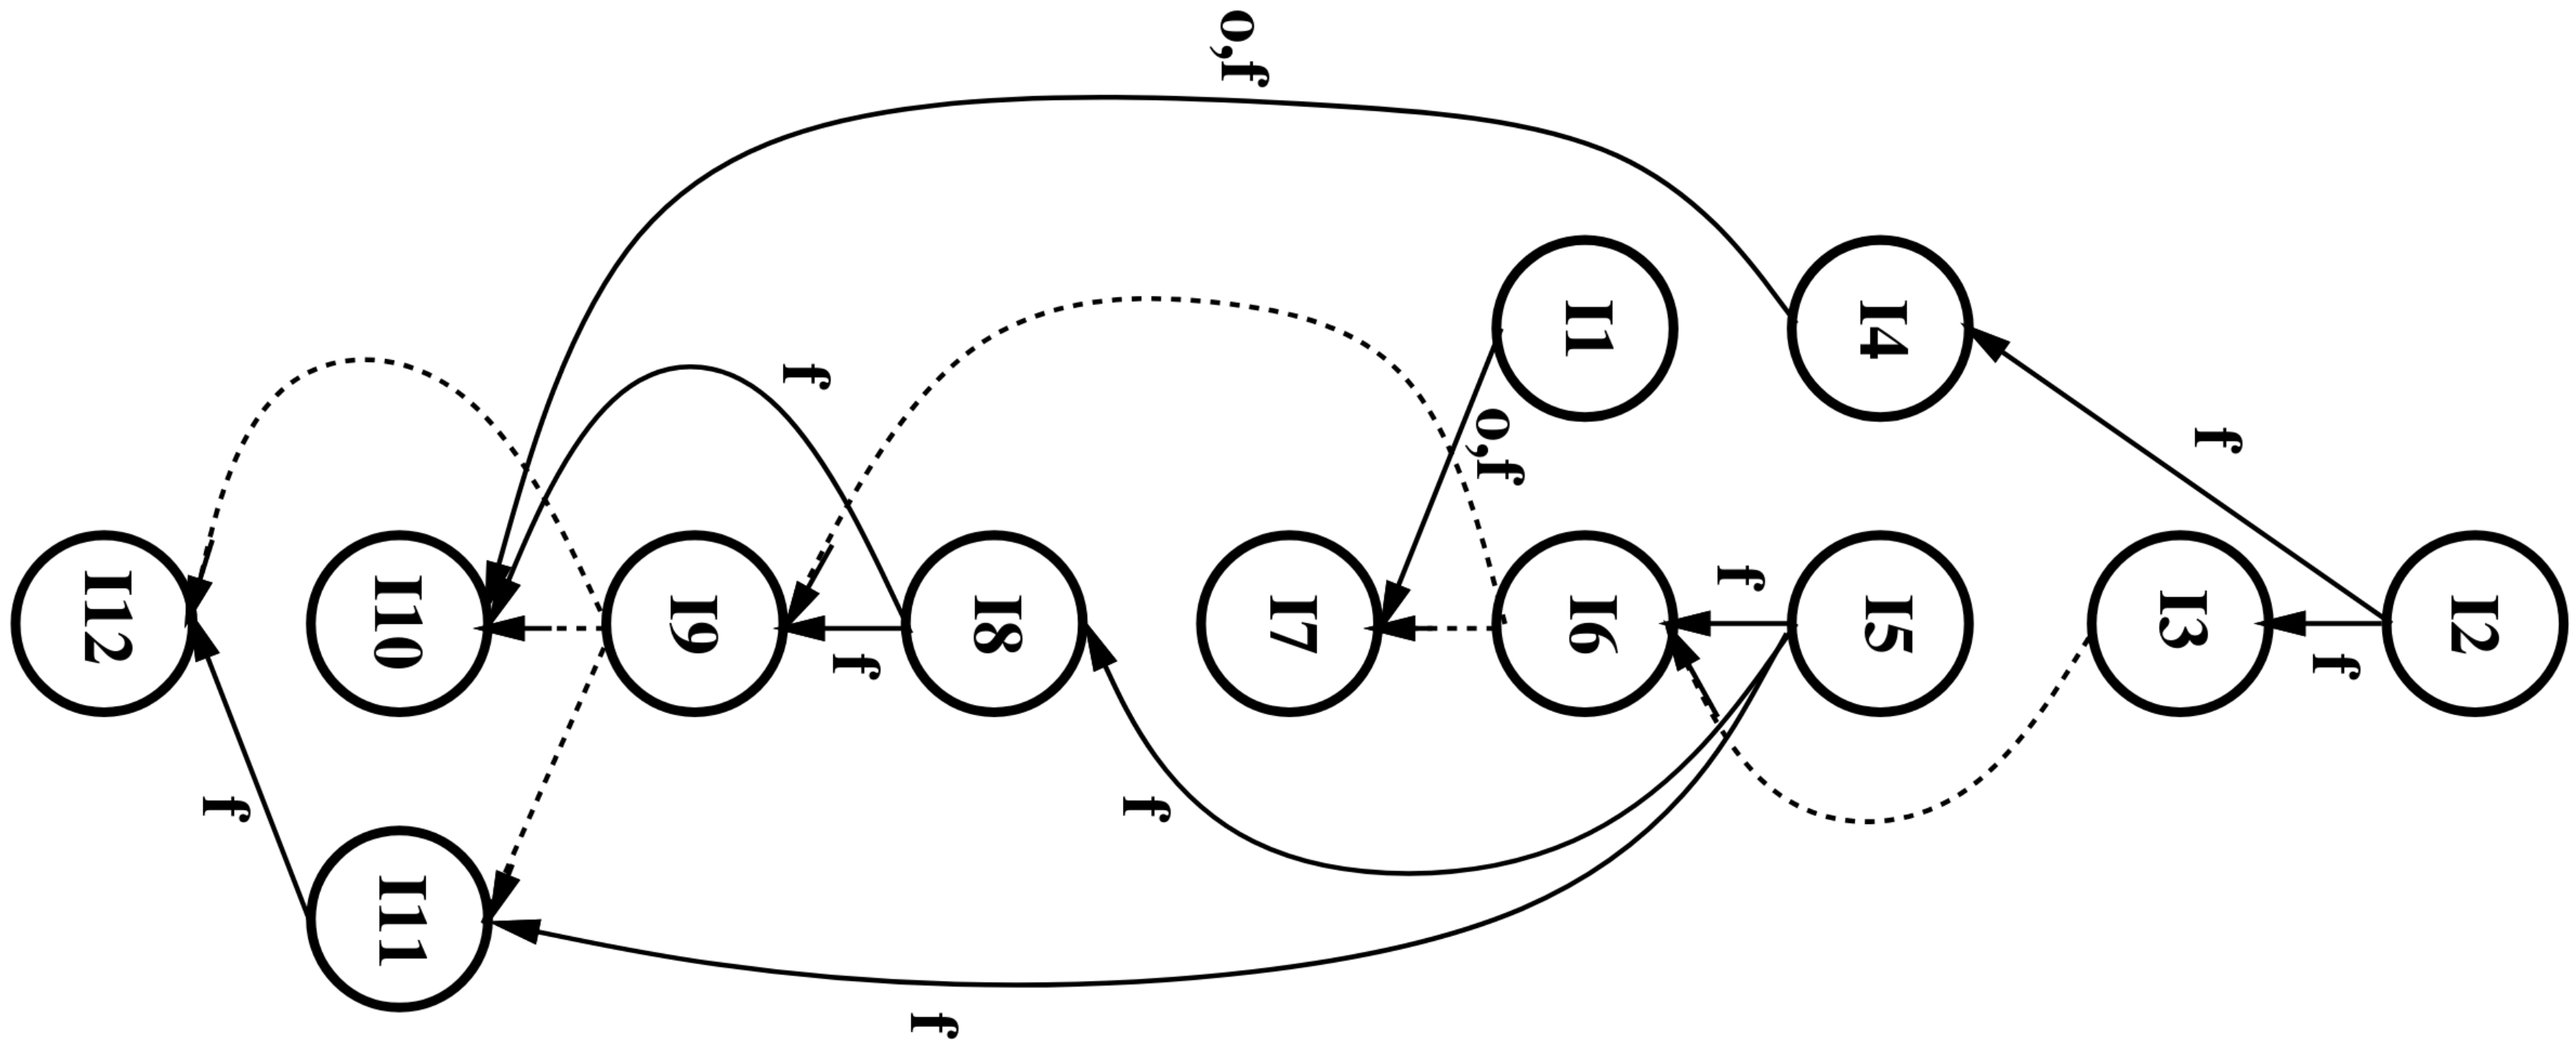
\includegraphics[width=\linewidth, angle=90]{src/figure/image/general_cfg.png}

            \caption{If we boost above one branch, we have three control dependencies left~\cite{chang95}.}
            \label{fig:boosting_cfg}
    \end{figure}
    \end{minipage}\hfill
    \begin{minipage}{.46\textwidth}
    \begin{figure}[H]
            \centering
            \resizebox{1\textwidth}{!}{
            \begin{tikzpicture}[font=\sffamily, scale=1]
\def\cellwidth{1.8}
\def\cellheight{0.8}

%\newlength{\cellwidthLength}
\setlength{\cellwidthLength}{\cellwidth cm}
%\newlength{\cellheightLength}
\setlength{\cellheightLength}{\cellheight cm}

\tikzstyle{ALU} = [fill=orange!20, draw=black, rectangle, minimum width=\cellwidthLength, minimum height=\cellheightLength]
\tikzstyle{LOAD} = [fill=orange!20, draw=black, rectangle, minimum width=\cellwidthLength, minimum height=\cellheightLength]
\tikzstyle{BRANCH} = [fill=purple!20, draw=black, rectangle, minimum width=\cellwidthLength, minimum height=\cellheightLength]
\tikzstyle{EMPTY} = [fill=gray!20, draw=black, rectangle, minimum width=\cellwidthLength, minimum height=\cellheightLength]

\def\numcycles{5}
\def\numunits{4}

\foreach \i in {1,...,\numcycles} {
    \foreach \j in {1,...,\numunits} {
        \pgfmathsetmacro{\x}{(\j - 1) * \cellwidth}
        \pgfmathsetmacro{\y}{-\i * \cellheight}
        \draw[EMPTY] (\x cm, \y cm) rectangle ++(\cellwidthLength, \cellheightLength);
    }
}

\foreach \j in {1,...,\numunits} {
    \pgfmathsetmacro{\x}{(\j - 1) * \cellwidth + 0.5 * \cellwidth}
    \node at (\x cm, 0.5 * \cellheight cm) {\small\textbf{U \j}};
}

\foreach \i in {1,...,\numcycles} {
    \pgfmathsetmacro{\y}{-\i * \cellheight + 0.5 * \cellheight}
    \node[anchor=east] at (-0.2 cm, \y cm) {\small\textbf{C\i}};
}

% Cycle 1
\pgfmathsetmacro{\y}{-1 * \cellheight}
\draw[ALU] (0 cm, \y cm) rectangle ++(\cellwidthLength, \cellheightLength) node[pos=.5] {\small I-1 add};
\draw[LOAD] (\cellwidth cm, \y cm) rectangle ++(\cellwidthLength, \cellheightLength) node[pos=.5] {\small I-2 ldr};
\draw[LOAD] (2 * \cellwidth cm, \y cm) rectangle ++(\cellwidthLength, \cellheightLength) node[pos=.5] {\small I-5 ldr};

% Cycle 2
\pgfmathsetmacro{\y}{-2 * \cellheight}
\draw[ALU] (0 cm, \y cm) rectangle ++(\cellwidthLength, \cellheightLength) node[pos=.5] {\small I-7 add};

% Cycle 3
\pgfmathsetmacro{\y}{-3 * \cellheight}
\draw[BRANCH] (0 cm, \y cm) rectangle ++(\cellwidthLength, \cellheightLength) node[pos=.5] {\small I-3 btl};
\draw[ALU] (\cellwidth cm, \y cm) rectangle ++(\cellwidthLength, \cellheightLength) node[pos=.5] {\small I-4 add};
\draw[LOAD] (2 * \cellwidth cm, \y cm) rectangle ++(\cellwidthLength, \cellheightLength) node[pos=.5] {\small I-8 ldr};
\draw[LOAD] (3 * \cellwidth cm, \y cm) rectangle ++(\cellwidthLength, \cellheightLength) node[pos=.5] {\small I-11 ldr};

% Cycle 4
\pgfmathsetmacro{\y}{-4 * \cellheight}
\draw[BRANCH] (0 cm, \y cm) rectangle ++(\cellwidthLength, \cellheightLength) node[pos=.5] {\small I-6 beq};

% Cycle 5
\pgfmathsetmacro{\y}{-5 * \cellheight}
\draw[BRANCH] (0 cm, \y cm) rectangle ++(\cellwidthLength, \cellheightLength) node[pos=.5] {\small I-9 btl};
\draw[ALU] (\cellwidth cm, \y cm) rectangle ++(\cellwidthLength, \cellheightLength) node[pos=.5] {\small I-10 add};
\draw[BRANCH] (2 *\cellwidth cm, \y cm) rectangle ++(\cellwidthLength, \cellheightLength) node[pos=.5] {\small I-12 bne};


\foreach \i in {1,...,\numcycles} {
    \foreach \j in {1,...,\numunits} {
        \pgfmathsetmacro{\x}{(\j - 1) * \cellwidth}
        \pgfmathsetmacro{\y}{-\i * \cellheight}
        \draw (\x cm, \y cm) rectangle ++(\cellwidthLength, \cellheightLength);
    }
}

\end{tikzpicture} 
        }
        \caption{\texttt{I7} can be scheduled in \texttt{C2}. The incremented \texttt{count} variable will be copied into the real register once branch \texttt{I6} commits and was not taken.}
        \label{fig:boosted_motion}
    \end{figure}
    \end{minipage}
    \end{center} 
\end{frame}

\begin{frame}{Practical Study}
    \begin{center}
        \resizebox{0.65\columnwidth}{!}{
            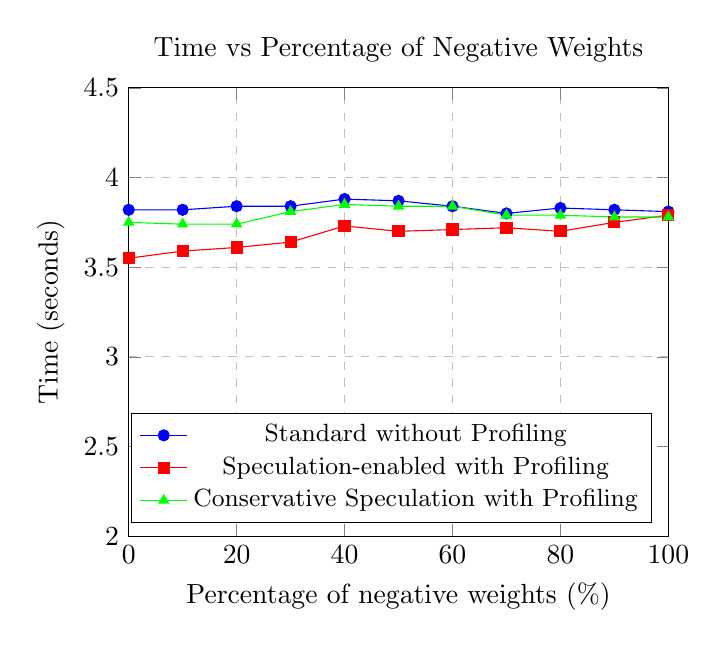
\begin{tikzpicture}
\begin{axis}[
    title={Time vs Percentage of Negative Weights},
    xlabel={Percentage of negative weights (\%)},
    ylabel={Time (seconds)},
    xmin=0, xmax=100,
    ymin=2, ymax=4.5,
    xtick={0,20,40,60,80,100},
    ytick={2,2.5,3,3.5,4,4.5},
    legend pos=south east,
    legend style={font=\small},
    ymajorgrids=true,
    xmajorgrids=true,
    grid style=dashed,
]

\addplot[color=blue, mark=*] coordinates {
    (0, 3.82)
    (10, 3.82)
    (20, 3.84)
    (30, 3.84)
    (40, 3.88)
    (50, 3.87)
    (60, 3.84)
    (70, 3.80)
    (80, 3.83)
    (90, 3.82)
    (100, 3.81)
};
\addlegendentry{Standard without Profiling}

\addplot[color=red, mark=square*] coordinates {
    (0, 3.55)
    (10, 3.59)
    (20, 3.61)
    (30, 3.64)
    (40, 3.73)
    (50, 3.70)
    (60, 3.71)
    (70, 3.72)
    (80, 3.70)
    (90, 3.75)
    (100, 3.79)
};
\addlegendentry{Speculation-enabled with Profiling}

\addplot[color=green, mark=triangle*] coordinates {
    (0, 3.75)
    (10, 3.74)
    (20, 3.74)
    (30, 3.81)
    (40, 3.85)
    (50, 3.84)
    (60, 3.84)
    (70, 3.79)
    (80, 3.79)
    (90, 3.78)
    (100, 3.78)
};
\addlegendentry{Conservative Speculation with Profiling}

\end{axis}
\end{tikzpicture}

        }
        \captionof{figure}{99\% positive weights during profiling, increasing percentage of negative weight during benchmarking.}
    \end{center} 
\end{frame}

\begin{frame}{Predication}
    \centering
    \LARGE Many branches are hard to predict.
\end{frame}

\begin{frame}{Predicated Instructions}
\begin{center}
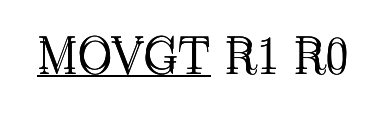
\begin{tikzpicture}[
    every node/.style={font=\large},
]
    \node<1> (movgt1) {%
        {\LARGE MOVGT R1 R0}%
    };
    \node<2> (movgt2) {%
        {\LARGE \underline{MOV}GT R1 R0}%
    };
    \node<3> (movgt3) {%
        {\LARGE MOV\underline{GT} R1 R0}%
    };
    \node<4> (movgt4) {%
        {\LARGE MOVGT R1 R0}%
    };

\end{tikzpicture}
\end{center}
\end{frame}

\begin{frame}{Minimal Predication Example}
    \only<1>{% First view
        \begin{figure}
        \begin{tabular}{ c c c c }
\adjustbox{valign=m}{%
\begin{lstlisting}[language=C++, basicstyle=\ttfamily\small]
if (x > 0) y = 10;
else y = 20;
\end{lstlisting}
}
&
\adjustbox{valign=m}{%
\begin{tikzpicture}
    \draw[->, line width=0.5pt, white] (0,0.5) -- (2, 1.5);
    \draw[->, line width=0.5pt, white] (0,-0.5) -- (2, -1.5);
\end{tikzpicture}
}
&
\adjustbox{valign=m}{%
\begin{minipage}{0.4\textwidth}
\textbf{\textcolor{white}{Without If-Conversion:}}
\begin{lstlisting}[
    basicstyle=\ttfamily\small\color{white}, 
    keywordstyle=\color{white}, 
    commentstyle=\color{white}, 
    stringstyle=\color{white}, 
    numbers=none
]
    cmp r0, #0
    bgt greater
    mov r1, #20
    b end
greater:
    mov r1, #10
end:
\end{lstlisting}


\vspace{0.8cm} % Space between the two assembly listings

\textbf{\textcolor{white}{With If-Conversion:}}
\begin{lstlisting}[
    basicstyle=\ttfamily\small\color{white}, 
    keywordstyle=\color{white}, 
    commentstyle=\color{white}, 
    stringstyle=\color{white}, 
    numbers=none
]
    cmp r0, #0
    movgt r1, #10
    movle r1, #20
\end{lstlisting}
\end{minipage}
}
\end{tabular}
        \end{figure}
    }
    \only<2>{% Second view
        \begin{figure}
        \begin{tabular}{ c c c c }
\adjustbox{valign=m}{%
\begin{lstlisting}[language=C++, basicstyle=\ttfamily\small]
if (x > 0) y = 10;
else y = 20;
\end{lstlisting}
}
&
\adjustbox{valign=m}{%
\begin{tikzpicture}
    \draw[->, line width=0.5pt] (0,0.5) -- (2, 1.5);
    \draw[->, line width=0.5pt, white] (0,-0.5) -- (2, -1.5);
\end{tikzpicture}
}
&
\adjustbox{valign=m}{%
\begin{minipage}{0.4\textwidth}
\textbf{Before If-Conversion:}
\begin{lstlisting}[
    basicstyle=\ttfamily\small, 
    numbers=none
]
    cmp r0, #0
    bgt greater
    mov r1, #20
    b end
greater:
    mov r1, #10
end:
\end{lstlisting}


\vspace{0.8cm} % Space between the two assembly listings

\textbf{\textcolor{white}{With If-Conversion:}}
\begin{lstlisting}[
    basicstyle=\ttfamily\small\color{white}, 
    keywordstyle=\color{white}, 
    commentstyle=\color{white}, 
    stringstyle=\color{white}, 
    numbers=none
]
    cmp r0, #0
    movgt r1, #10
    movle r1, #20
\end{lstlisting}
\end{minipage}
}
\end{tabular}
        \end{figure}
    }
    \only<3>{% Third view
        \begin{figure}
        \begin{tabular}{ c c c c }
\adjustbox{valign=m}{%
\begin{lstlisting}[language=C++, basicstyle=\ttfamily\small]
if (x > 0) y = 10;
else y = 20;
\end{lstlisting}
}
&
\adjustbox{valign=m}{%
\begin{tikzpicture}
    \draw[->, line width=0.5pt] (0,0.5) -- (2, 1.5);
    \draw[->, line width=0.5pt] (0,-0.5) -- (2, -1.5);
\end{tikzpicture}
}
&
\adjustbox{valign=m}{%
\begin{minipage}{0.4\textwidth}
\textbf{Without Predication:}
\begin{lstlisting}[basicstyle=\ttfamily\small]
    cmp r0, #0
    bgt greater
    mov r1, #20
    b end
greater:
    mov r1, #10
end:
\end{lstlisting}

\vspace{0.8cm} % Space between the two assembly listings

\textbf{With Predication:}
\begin{lstlisting}[basicstyle=\ttfamily\small]
    cmp r0, #0
    movgt r1, #10
    movle r1, #20
\end{lstlisting}
\end{minipage}
}
\end{tabular}
        \end{figure}
    }
\end{frame}

\begin{frame}[fragile]
\frametitle{Predication}
\begin{center}
    \scalebox{0.95}{          
        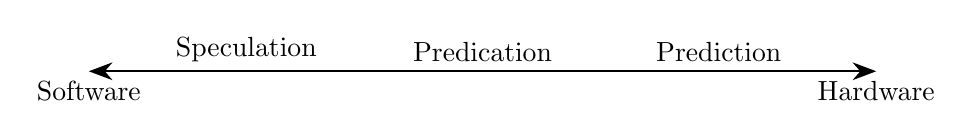
\begin{tikzpicture}[align=center]
        
        \draw[arrows={Stealth[length=3mm]-Stealth[length=3mm]}, thick] (0,0) -- (10,0);
        
        % Place labels at the ends
        \node[below] at (0,0) {Software};
        \node[below] at (10,0) {Hardware};
        
        \node[above] at (2,0) {Speculation};
        \node[above] at (5,0) {Predication};
        \node[above] at (8,0) {Prediction};
        
        \end{tikzpicture}
    }
\end{center}
\end{frame}

\begin{frame}{ARMv7 Predication}
\centering
    {\LARGE MOVGT vs MOV}
    \only<1>{
        \begin{center}
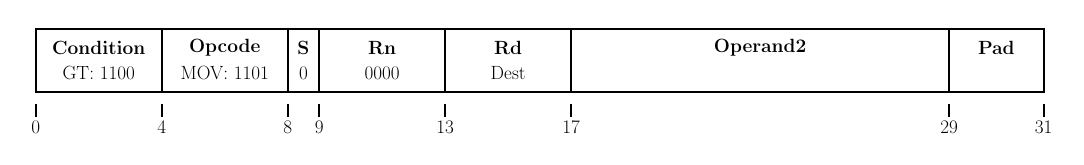
\begin{tikzpicture}[scale=0.4, every node/.style={scale=0.4}]
    % Bit fields with adjusted widths and labels for clarity
    \draw[thick] (0,0) rectangle (4,2) node[midway, yshift=0.4cm] {\textbf{\LARGE Condition}};
    \node at (2, 0.6) {\LARGE GT: 1100};
    
    \draw[thick] (4,0) rectangle (8,2) node[midway, yshift=0.4cm] {\textbf{\LARGE Opcode}};
    \node at (6, 0.6) {\LARGE MOV: 1101};
    
    \draw[thick] (8,0) rectangle (9,2) node[midway, yshift=0.4cm] {\textbf{\LARGE S}};
    \node at (8.5, 0.6) {\LARGE 0};
    
    \draw[thick] (9,0) rectangle (13,2) node[midway, yshift=0.4cm] {\textbf{\LARGE Rn}};
    \node at (11, 0.6) {\LARGE 0000};
    
    \draw[thick] (13,0) rectangle (17,2) node[midway, yshift=0.4cm] {\textbf{\LARGE Rd}};
    \node at (15, 0.6) {\LARGE Dest};
    
    \draw[thick] (17,0) rectangle (29,2) node[midway, yshift=0.4cm] {\textbf{\LARGE Operand2}};
    
    \draw[thick] (29,0) rectangle (32,2) node[midway, yshift=0.4cm] {\textbf{\LARGE Pad}};
    
    % Bit numbers
    \draw[thick] (0,-0.4) -- (0,-0.8) node[below] {\LARGE 0};
    \draw[thick] (4,-0.4) -- (4,-0.8) node[below] {\LARGE 4};
    \draw[thick] (8,-0.4) -- (8,-0.8) node[below] {\LARGE 8};
    \draw[thick] (9,-0.4) -- (9,-0.8) node[below] {\LARGE 9};
    \draw[thick] (13,-0.4) -- (13,-0.8) node[below] {\LARGE 13};
    \draw[thick] (17,-0.4) -- (17,-0.8) node[below] {\LARGE 17};
    \draw[thick] (29,-0.4) -- (29,-0.8) node[below] {\LARGE 29};
    \draw[thick] (32,-0.4) -- (32,-0.8) node[below] {\LARGE 31};

\end{tikzpicture}
\end{center}
        \begin{center}
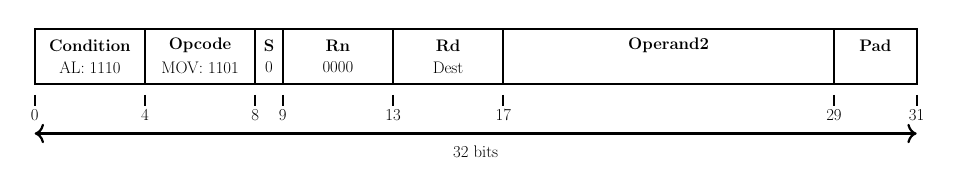
\begin{tikzpicture}[scale=0.35, every node/.style={scale=0.35}]
    % Bit fields with adjusted widths and labels for clarity
    \draw[thick] (0,0) rectangle (4,2) node[midway, yshift=0.4cm] {\textbf{\LARGE Condition}};
    \node at (2, 0.6) {\LARGE AL: 1110};
    
    \draw[thick] (4,0) rectangle (8,2) node[midway, yshift=0.4cm] {\textbf{\LARGE Opcode}};
    \node at (6, 0.6) {\LARGE MOV: 1101};
    
    \draw[thick] (8,0) rectangle (9,2) node[midway, yshift=0.4cm] {\textbf{\LARGE S}};
    \node at (8.5, 0.6) {\LARGE 0};
    
    \draw[thick] (9,0) rectangle (13,2) node[midway, yshift=0.4cm] {\textbf{\LARGE Rn}};
    \node at (11, 0.6) {\LARGE 0000};
    
    \draw[thick] (13,0) rectangle (17,2) node[midway, yshift=0.4cm] {\textbf{\LARGE Rd}};
    \node at (15, 0.6) {\LARGE Dest};
    
    \draw[thick] (17,0) rectangle (29,2) node[midway, yshift=0.4cm] {\textbf{\LARGE Operand2}};
    
    \draw[thick] (29,0) rectangle (32,2) node[midway, yshift=0.4cm] {\textbf{\LARGE Pad}};
    
    % Bit numbers
    \draw[thick] (0,-0.4) -- (0,-0.8) node[below] {\LARGE 0};
    \draw[thick] (4,-0.4) -- (4,-0.8) node[below] {\LARGE 4};
    \draw[thick] (8,-0.4) -- (8,-0.8) node[below] {\LARGE 8};
    \draw[thick] (9,-0.4) -- (9,-0.8) node[below] {\LARGE 9};
    \draw[thick] (13,-0.4) -- (13,-0.8) node[below] {\LARGE 13};
    \draw[thick] (17,-0.4) -- (17,-0.8) node[below] {\LARGE 17};
    \draw[thick] (29,-0.4) -- (29,-0.8) node[below] {\LARGE 29};
    \draw[thick] (32,-0.4) -- (32,-0.8) node[below] {\LARGE 31};

    % Arrow for full bit length label
    \draw[<->, thick] (0,-1.8) -- (32,-1.8) node[midway, below, yshift=-0.3cm] {\LARGE 32 bits};
\end{tikzpicture}
\end{center}

    }
    \only<2>{
        \begin{center}
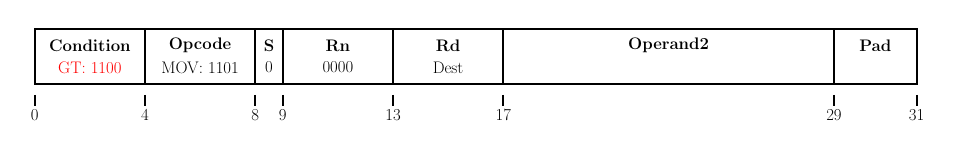
\begin{tikzpicture}[scale=0.35, every node/.style={scale=0.35}]
    % Bit fields with adjusted widths and labels for clarity
    \draw[thick] (0,0) rectangle (4,2) node[midway, yshift=0.4cm] {\textbf{\LARGE Condition}};
    \node at (2, 0.6) {\textcolor{red}{\LARGE GT: 1100}};
    
    \draw[thick] (4,0) rectangle (8,2) node[midway, yshift=0.4cm] {\textbf{\LARGE Opcode}};
    \node at (6, 0.6) {\LARGE MOV: 1101};
    
    \draw[thick] (8,0) rectangle (9,2) node[midway, yshift=0.4cm] {\textbf{\LARGE S}};
    \node at (8.5, 0.6) {\LARGE 0};
    
    \draw[thick] (9,0) rectangle (13,2) node[midway, yshift=0.4cm] {\textbf{\LARGE Rn}};
    \node at (11, 0.6) {\LARGE 0000};
    
    \draw[thick] (13,0) rectangle (17,2) node[midway, yshift=0.4cm] {\textbf{\LARGE Rd}};
    \node at (15, 0.6) {\LARGE Dest};
    
    \draw[thick] (17,0) rectangle (29,2) node[midway, yshift=0.4cm] {\textbf{\LARGE Operand2}};
    
    \draw[thick] (29,0) rectangle (32,2) node[midway, yshift=0.4cm] {\textbf{\LARGE Pad}};
    
    % Bit numbers
    \draw[thick] (0,-0.4) -- (0,-0.8) node[below] {\LARGE 0};
    \draw[thick] (4,-0.4) -- (4,-0.8) node[below] {\LARGE 4};
    \draw[thick] (8,-0.4) -- (8,-0.8) node[below] {\LARGE 8};
    \draw[thick] (9,-0.4) -- (9,-0.8) node[below] {\LARGE 9};
    \draw[thick] (13,-0.4) -- (13,-0.8) node[below] {\LARGE 13};
    \draw[thick] (17,-0.4) -- (17,-0.8) node[below] {\LARGE 17};
    \draw[thick] (29,-0.4) -- (29,-0.8) node[below] {\LARGE 29};
    \draw[thick] (32,-0.4) -- (32,-0.8) node[below] {\LARGE 31};

\end{tikzpicture}
\end{center}
        \begin{center}
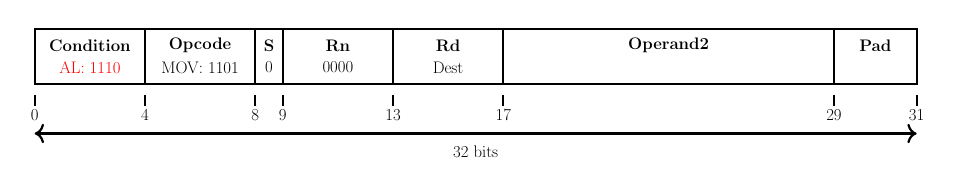
\begin{tikzpicture}[scale=0.35, every node/.style={scale=0.35}]
    % Bit fields with adjusted widths and labels for clarity
    \draw[thick] (0,0) rectangle (4,2) node[midway, yshift=0.4cm] {\textbf{\LARGE Condition}};
    \node at (2, 0.6) {\textcolor{red}{\LARGE AL: 1110}};
    
    \draw[thick] (4,0) rectangle (8,2) node[midway, yshift=0.4cm] {\textbf{\LARGE Opcode}};
    \node at (6, 0.6) {\LARGE MOV: 1101};
    
    \draw[thick] (8,0) rectangle (9,2) node[midway, yshift=0.4cm] {\textbf{\LARGE S}};
    \node at (8.5, 0.6) {\LARGE 0};
    
    \draw[thick] (9,0) rectangle (13,2) node[midway, yshift=0.4cm] {\textbf{\LARGE Rn}};
    \node at (11, 0.6) {\LARGE 0000};
    
    \draw[thick] (13,0) rectangle (17,2) node[midway, yshift=0.4cm] {\textbf{\LARGE Rd}};
    \node at (15, 0.6) {\LARGE Dest};
    
    \draw[thick] (17,0) rectangle (29,2) node[midway, yshift=0.4cm] {\textbf{\LARGE Operand2}};
    
    \draw[thick] (29,0) rectangle (32,2) node[midway, yshift=0.4cm] {\textbf{\LARGE Pad}};
    
    % Bit numbers
    \draw[thick] (0,-0.4) -- (0,-0.8) node[below] {\LARGE 0};
    \draw[thick] (4,-0.4) -- (4,-0.8) node[below] {\LARGE 4};
    \draw[thick] (8,-0.4) -- (8,-0.8) node[below] {\LARGE 8};
    \draw[thick] (9,-0.4) -- (9,-0.8) node[below] {\LARGE 9};
    \draw[thick] (13,-0.4) -- (13,-0.8) node[below] {\LARGE 13};
    \draw[thick] (17,-0.4) -- (17,-0.8) node[below] {\LARGE 17};
    \draw[thick] (29,-0.4) -- (29,-0.8) node[below] {\LARGE 29};
    \draw[thick] (32,-0.4) -- (32,-0.8) node[below] {\LARGE 31};

    % Arrow for full bit length label
    \draw[<->, thick] (0,-1.8) -- (32,-1.8) node[midway, below, yshift=-0.3cm] {\LARGE 32 bits};
\end{tikzpicture}
\end{center}

    }
\end{frame}

\begin{frame}{If-converting a real function}
    \only<1>{
    \begin{figure}
        \centering
        \end{figure}    
    }
    \only<2>{
    \begin{figure}
        \centering
        \begin{minipage}{0.50\textwidth}
    \begin{lstlisting}[style=CStyle, basicstyle=\tiny\ttfamily]
#include <cstdint>

uint32_t 
computeLoan(bool isHouseLoan, int principal) 
{
  //EBB
  uint32_t baseRate = principal * 2 / 100;

  if (isHouseLoan) {
    // TBB
    baseRate = principal * 5 / 100;
  } else {
    // FBB
    baseRate = principal * 7 / 100;
  }

  // TailBB
  return (baseRate + 5) / 10 * 10;
}
    \end{lstlisting}
\end{minipage}%
\hspace{1cm} % Adjust horizontal overlap
\begin{minipage}{0.40\textwidth}
\begin{tikzpicture}[node distance=2cm and 3cm, >=stealth]
    % Style for consistent node dimensions
    \tikzstyle{node} = [circle, draw, white, minimum size=1.5cm, inner sep=0]

    % Nodes
    \node[node] (EBB) at (1.5, 4.5) {EBB};
    \node[node] (TBB) at (3, 2.25) {TBB};
    \node[node] (FBB) at (0, 2.25) {FBB};
    \node[node] (TailBB) at (1.5, 0) {TailBB};

    % Edges

\end{tikzpicture}
\end{minipage}
        \end{figure}    
    }
    \only<3> {
        \begin{figure}
        \centering
        \begin{minipage}{0.50\textwidth}
    \begin{lstlisting}[style=CStyle]
#include <cstdint>

uint32_t 
computeLoan(bool isHouseLoan, 
                int principal) {
  //EBB
  uint32_t
  baseRate = principal * 2 / 100;

  if (isHouseLoan) {
    // TBB
    baseRate = principal * 5 / 100;
  } else {
    // FBB
    baseRate = principal * 7 / 100;
  }

  // TailBB
  return (baseRate + 5) / 10 * 10;
}
    \end{lstlisting}
\end{minipage}%
\hspace{1cm} % Adjust horizontal overlap
\begin{minipage}{0.40\textwidth}
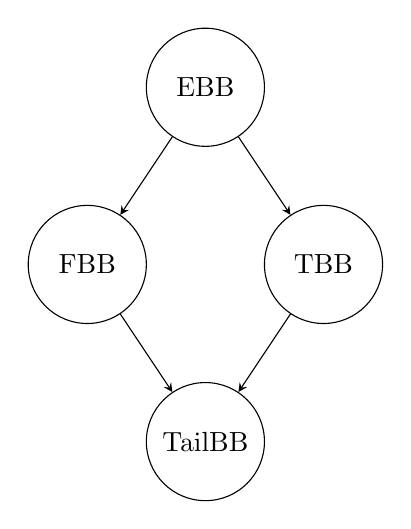
\begin{tikzpicture}[node distance=2cm and 3cm, >=stealth]
    % Style for consistent node dimensions
    \tikzstyle{node} = [circle, draw, fill=white, minimum size=1.5cm, inner sep=0]

    % Nodes
    \node[node] (EBB) at (1.5, 4.5) {EBB};
    \node[node] (TBB) at (3, 2.25) {TBB};
    \node[node] (FBB) at (0, 2.25) {FBB};
    \node[node] (TailBB) at (1.5, 0) {TailBB};

    % Edges
    \draw[->] (EBB) -- (TBB);
    \draw[->] (EBB) -- (FBB);
    \draw[->] (TBB) -- (TailBB);
    \draw[->] (FBB) -- (TailBB);
\end{tikzpicture}
\end{minipage}
        \end{figure}   
    }
\end{frame}

\begin{frame}{If-converting a real function}
    \only<1>{% First view
        \begin{figure}
            \centering
            \begin{minipage}{0.45\textwidth}
    \begin{lstlisting}[style=AsmStyle, basicstyle=\fontsize{4}{5}\selectfont\ttfamily]
computeLoan(bool, int):
    push    {r11, lr}
    mov     r11, sp
    sub     sp, sp, #16
    and     r0, r0, #1
    strb    r0, [r11, #-1]
    str     r1, [sp, #8]
    ldr     r0, [sp, #8]
    lsl     r0, r0, #1
    ldr     r1, .LCPI0_0
    bl      __aeabi_idiv
    str     r0, [sp, #4]
    ldrb    r0, [r11, #-1]
    tst     r0, #1
    beq     .LBB0_2
    ldr     r0, [sp, #8]
    ldr     r1, .LCPI0_3
    mul     r0, r0, r1
    ldr     r1, .LCPI0_0
    bl      __aeabi_idiv
    str     r0, [sp, #4]
    b       .LBB0_3
.LBB0_2:
    ldr     r0, [sp, #8]
    ldr     r1, .LCPI0_2
    mul     r0, r0, r1
    ldr     r1, .LCPI0_0
    bl      __aeabi_idiv
    str     r0, [sp, #4]
.LBB0_3:
    ldr     r0, [sp, #4]
    add     r0, r0, #5
    ldr     r1, .LCPI0_4
    bl      __aeabi_uidiv
    ldr     r1, .LCPI0_4
    mul     r0, r0, r1
    mov     sp, r11
    pop     {r11, pc}
    \end{lstlisting}
\end{minipage}%
\hspace{1cm}
\begin{minipage}{0.45\textwidth}
    \begin{lstlisting}[numbers=right, basicstyle=\fontsize{4}{5}\selectfont\ttfamily\color{white}, belowskip=8.5\baselineskip]
computeLoan(bool, int):
    push    {r11, lr}
    mov     r11, sp
    sub     sp, sp, #16
    and     r0, r0, #1
    strb    r0, [r11, #-1]
    str     r1, [sp, #8]
    ldr     r0, [sp, #8]
    lsl     r0, r0, #1
    ldr     r1, .LCPI0_0
    bl      __aeabi_idiv
    str     r0, [sp, #4]
    ldrb    r0, [r11, #-1]
    ldr     r3, .LCPI0_3
    ldr     r4, .LCPI0_2
    cmp     r0, #1
    mov     r1, r3
    movne   r1, r4
    ldr     r0, [sp, #8]
    mul     r0, r0, r1
    ldr     r1, .LCPI0_0
    bl      __aeabi_idiv
    str     r0, [sp, #4]
    ldr     r0, [sp, #4]
    add     r0, r0, #5
    ldr     r1, .LCPI0_4
    bl      __aeabi_uidiv
    ldr     r1, .LCPI0_4
    mul     r0, r0, r1
    mov     sp, r11
    pop     {r11, pc} 
    \end{lstlisting}
\end{minipage}%

        \end{figure}
    }
    \only<2>{% Second view
        \begin{figure}
            \centering
            \begin{minipage}{0.45\textwidth}
    \begin{lstlisting}[style=AsmStyle, basicstyle=\fontsize{4}{5}\selectfont\ttfamily]
computeLoan(bool, int):
    push    {r11, lr}
    mov     r11, sp
    sub     sp, sp, #16
    and     r0, r0, #1
    strb    r0, [r11, #-1]
    str     r1, [sp, #8]
    ldr     r0, [sp, #8]
    lsl     r0, r0, #1
    ldr     r1, .LCPI0_0
    bl      __aeabi_idiv
    str     r0, [sp, #4]
    ldrb    r0, [r11, #-1]
    tst     r0, #1
    beq     .LBB0_2
    ldr     r0, [sp, #8]
    ldr     r1, .LCPI0_3
    mul     r0, r0, r1
    ldr     r1, .LCPI0_0
    bl      __aeabi_idiv
    str     r0, [sp, #4]
    b       .LBB0_3
.LBB0_2:
    ldr     r0, [sp, #8]
    ldr     r1, .LCPI0_2
    mul     r0, r0, r1
    ldr     r1, .LCPI0_0
    bl      __aeabi_idiv
    str     r0, [sp, #4]
.LBB0_3:
    ldr     r0, [sp, #4]
    add     r0, r0, #5
    ldr     r1, .LCPI0_4
    bl      __aeabi_uidiv
    ldr     r1, .LCPI0_4
    mul     r0, r0, r1
    mov     sp, r11
    pop     {r11, pc}
    \end{lstlisting}
\end{minipage}%
\hspace{1cm}
\begin{minipage}{0.45\textwidth}
    \begin{lstlisting}[style=AsmStyle, numbers=right,  basicstyle=\fontsize{4}{5}\selectfont\ttfamily, belowskip=8.5\baselineskip]
computeLoan(bool, int):
    push    {r11, lr}
    mov     r11, sp
    sub     sp, sp, #16
    and     r0, r0, #1
    strb    r0, [r11, #-1]
    str     r1, [sp, #8]
    ldr     r0, [sp, #8]
    lsl     r0, r0, #1
    ldr     r1, .LCPI0_0
    bl      __aeabi_idiv
    str     r0, [sp, #4]
    ldrb    r0, [r11, #-1]
    ldr     r3, .LCPI0_3
    ldr     r4, .LCPI0_2
    cmp     r0, #1
    mov     r1, r3
    movne   r1, r4
    ldr     r0, [sp, #8]
    mul     r0, r0, r1
    ldr     r1, .LCPI0_0
    bl      __aeabi_idiv
    str     r0, [sp, #4]
    ldr     r0, [sp, #4]
    add     r0, r0, #5
    ldr     r1, .LCPI0_4
    bl      __aeabi_uidiv
    ldr     r1, .LCPI0_4
    mul     r0, r0, r1
    mov     sp, r11
    pop     {r11, pc} 
    \end{lstlisting}
\end{minipage}%

        \end{figure}
    }
    \only<3>{% Third view
        \begin{figure}
            \centering
            \begin{minipage}{0.45\textwidth}
    \begin{lstlisting}[style=AsmStyle, basicstyle=\fontsize{4}{5}\selectfont\ttfamily]
computeLoan(bool, int):
    push    {r11, lr}
    mov     r11, sp
    sub     sp, sp, #16
    and     r0, r0, #1
    strb    r0, [r11, #-1]
    str     r1, [sp, #8]
    ldr     r0, [sp, #8]
    lsl     r0, r0, #1
    ldr     r1, .LCPI0_0
    bl      __aeabi_idiv
    str     r0, [sp, #4]
    ldrb    r0, [r11, #-1]
    @tst     r0, #1
    @@beq     .LBB0_2
    ldr     r0, [sp, #8]
    ldr     r1, .LCPI0_3
    mul     r0, r0, r1
    ldr     r1, .LCPI0_0
    bl      __aeabi_idiv
    str     r0, [sp, #4]
    b       .LBB0_3
.LBB0_2:
    ldr     r0, [sp, #8]
    ldr     r1, .LCPI0_2
    mul     r0, r0, r1
    ldr     r1, .LCPI0_0
    bl      __aeabi_idiv
    str     r0, [sp, #4]
.LBB0_3:
    ldr     r0, [sp, #4]
    add     r0, r0, #5
    ldr     r1, .LCPI0_4
    bl      __aeabi_uidiv
    ldr     r1, .LCPI0_4
    mul     r0, r0, r1
    mov     sp, r11
    pop     {r11, pc}
    \end{lstlisting}
\end{minipage}%
\hspace{1cm}
\begin{minipage}{0.45\textwidth}
    \begin{lstlisting}[style=AsmStyle, numbers=right,  basicstyle=\fontsize{4}{5}\selectfont\ttfamily, belowskip=8.5\baselineskip]
computeLoan(bool, int):
    push    {r11, lr}
    mov     r11, sp
    sub     sp, sp, #16
    and     r0, r0, #1
    strb    r0, [r11, #-1]
    str     r1, [sp, #8]
    ldr     r0, [sp, #8]
    lsl     r0, r0, #1
    ldr     r1, .LCPI0_0
    bl      __aeabi_idiv
    str     r0, [sp, #4]
    ldrb    r0, [r11, #-1]
    ldr     r3, .LCPI0_3
    ldr     r4, .LCPI0_2
    @cmp     r0, #1
    @@mov     r1, r3
    @@movne   r1, r4
    ldr     r0, [sp, #8]
    mul     r0, r0, r1
    ldr     r1, .LCPI0_0
    bl      __aeabi_idiv
    str     r0, [sp, #4]
    ldr     r0, [sp, #4]
    add     r0, r0, #5
    ldr     r1, .LCPI0_4
    bl      __aeabi_uidiv
    ldr     r1, .LCPI0_4
    mul     r0, r0, r1
    mov     sp, r11
    pop     {r11, pc} 
    \end{lstlisting}
\end{minipage}%

        \end{figure}
    }
    \only<4>{% Sixth view
        \begin{figure}
            \centering
            \begin{minipage}{0.45\textwidth}
    \begin{lstlisting}[style=AsmStyle, basicstyle=\fontsize{4}{5}\selectfont\ttfamily]
computeLoan(bool, int):
    push    {r11, lr}
    mov     r11, sp
    sub     sp, sp, #16
    and     r0, r0, #1
    strb    r0, [r11, #-1]
    str     r1, [sp, #8]
    ldr     r0, [sp, #8]
    lsl     r0, r0, #1
    ldr     r1, .LCPI0_0
    bl      __aeabi_idiv
    str     r0, [sp, #4]
    ldrb    r0, [r11, #-1]
    tst     r0, #1
    beq     .LBB0_2
    @ldr     r0, [sp, #8]
    @@ldr     r1, .LCPI0_3
    @@mul     r0, r0, r1
    @@ldr     r1, .LCPI0_0
    @@bl      __aeabi_idiv
    @@str     r0, [sp, #4]
    b       .LBB0_3
.LBB0_2:
    @@ldr     r0, [sp, #8]
    @@ldr     r1, .LCPI0_2
    @@mul     r0, r0, r1
    @@ldr     r1, .LCPI0_0
    @@bl      __aeabi_idiv
    @@str     r0, [sp, #4]
.LBB0_3:
    ldr     r0, [sp, #4]
    add     r0, r0, #5
    ldr     r1, .LCPI0_4
    bl      __aeabi_uidiv
    ldr     r1, .LCPI0_4
    mul     r0, r0, r1
    mov     sp, r11
    pop     {r11, pc}
    \end{lstlisting}
\end{minipage}%
\hspace{1cm}
\begin{minipage}{0.45\textwidth}
    \begin{lstlisting}[style=AsmStyle, numbers=right,  basicstyle=\fontsize{4}{5}\selectfont\ttfamily, belowskip=8.5\baselineskip]
computeLoan(bool, int):
    push    {r11, lr}
    mov     r11, sp
    sub     sp, sp, #16
    and     r0, r0, #1
    strb    r0, [r11, #-1]
    str     r1, [sp, #8]
    ldr     r0, [sp, #8]
    lsl     r0, r0, #1
    ldr     r1, .LCPI0_0
    bl      __aeabi_idiv
    str     r0, [sp, #4]
    ldrb    r0, [r11, #-1]
    ldr     r3, .LCPI0_3
    ldr     r4, .LCPI0_2
    cmp     r0, #1
    mov     r1, r3
    movne   r1, r4
    @ldr     r0, [sp, #8]
    @@mul     r0, r0, r1
    @@ldr     r1, .LCPI0_0
    @@bl      __aeabi_idiv
    @@str     r0, [sp, #4]
    ldr     r0, [sp, #4]
    add     r0, r0, #5
    ldr     r1, .LCPI0_4
    bl      __aeabi_uidiv
    ldr     r1, .LCPI0_4
    mul     r0, r0, r1
    mov     sp, r11
    pop     {r11, pc}
    \end{lstlisting}
\end{minipage}%

        \end{figure}
    }
\end{frame}

\begin{frame}{If-converting a real function, benchmarks}
    \only<1>{% First view (empty slide)
        % Intentionally left blank
    }
    \only<2>{% Second view
        \centering
\begin{tikzpicture}
    \begin{axis}[
        width=10cm,
        height=7.5cm,
        ybar,
        symbolic x coords={ComputeLoan, ProcessOrder},
        xtick=data,
        ylabel={IPC (Percentage)},
        ymin=0, ymax=150,
        nodes near coords,
        bar width=25pt,
        axis lines=left,
        enlarge x limits=0.5,
        ytick={0,25,50,75,100,125,150},
        every axis label/.append style={font=\normalsize},
        every axis tick label/.append style={font=\small},
        legend style={at={(0.5,-0.15)}, anchor=north, legend columns=-1}, % Adjust legend position
        legend cell align={left}
    ]
        \addplot[pattern=dots, pattern color=red] coordinates {(ComputeLoan, 100) (ProcessOrder, 100)};
        \addlegendentry{Baseline}
        
        \addplot[pattern=north east lines, pattern color=red] coordinates {(ComputeLoan, 105.93) (ProcessOrder, 112.5)};
        \addlegendentry{Ifconverted}
    \end{axis}
\end{tikzpicture}
\hfill
\begin{tikzpicture}
    \begin{axis}[
        width=10cm,
        height=7.5cm,
        ybar,
        symbolic x coords={ComputeLoan, ProcessOrder},
        xtick=data,
        ylabel={Total Cycles (Percentage)},
        ymin=0, ymax=150,
        nodes near coords,
        bar width=25pt,
        axis lines=left,
        enlarge x limits=0.5,
        ytick={0,25,50,75,100,125,150},
        every axis label/.append style={font=\normalsize},
        every axis tick label/.append style={font=\small},
        legend style={at={(0.5,-0.15)}, anchor=north, legend columns=-1}, % Adjust legend position
        legend cell align={left}
    ]
        \addplot[pattern=dots, pattern color=blue] coordinates {(ComputeLoan, 100) (ProcessOrder, 100)};
        \addlegendentry{Baseline}
        
        \addplot[pattern=north east lines, pattern color=blue] coordinates {(ComputeLoan, 75.36) (ProcessOrder, 42.91)};
        \addlegendentry{Ifconverted}
    \end{axis}
\end{tikzpicture}

    }
\end{frame}

\begin{frame}{Pros and Cons of Predication}
    \only<1>{% First view
        \begin{columns}[t] % The `[t]` aligns columns at the top
    \column{0.5\textwidth}
        \textbf{Pros}
        \begin{itemize}
            \setbeamertemplate{itemize items}{\textcolor{green}{$\uparrow$}}
            \item Reduces Code Size
            \setbeamertemplate{itemize items}{\textcolor{white}{\textbf{\boldmath$\Uparrow$}}}
            \item \textcolor{white}{Removes Branches}
            \begin{itemize}
                \setbeamertemplate{itemize items}{\textcolor{white}{$\bullet$}}
                \item  \textcolor{white}{Removes branch misprediction penalty}
                \item  \textcolor{white}{Improves IPC}
                \item  \textcolor{white}{Makes execution time predictable}
            \end{itemize}
        \end{itemize}

    \column{0.5\textwidth}

\end{columns}
    }
    \only<2>{% Second view
        \begin{columns}[t] % The `[t]` aligns columns at the top
    \column{0.5\textwidth}
        \textbf{Pros}
        \begin{itemize}
            \setbeamertemplate{itemize items}{\textcolor{green}{$\uparrow$}}
            \item Reduces Code Size
            \setbeamertemplate{itemize items}{\textcolor{green}{\textbf{\boldmath$\Uparrow$}}}
            \item Removes Branches
            \begin{itemize}
                \setbeamertemplate{itemize items}{\textcolor{white}{$\bullet$}}
                \item  \textcolor{white}{Removes branch misprediction penalty}
                \item  \textcolor{white}{Improves IPC}
                \item  \textcolor{white}{Makes execution time predictable}
            \end{itemize}
        \end{itemize}

    \column{0.5\textwidth}

\end{columns}
    }
    \only<3>{% Third view
        \begin{columns}[t] % The `[t]` aligns columns at the top
    \column{0.5\textwidth}
        \textbf{Pros}
        \begin{itemize}
            \setbeamertemplate{itemize items}{\textcolor{green}{$\uparrow$}}
            \item Reduces Code Size
            \setbeamertemplate{itemize items}{\textcolor{green}{\textbf{\boldmath$\Uparrow$}}}
            \item Removes Branches
            \begin{itemize}
                \setbeamertemplate{itemize items}{\textcolor{green}{$\bullet$}}
                \item Removes branch misprediction penalty
                \item Improves IPC
                \item Makes execution time predictable
            \end{itemize}
        \end{itemize}

    \column{0.5\textwidth}

\end{columns}
    }
    \only<4>{% Fourth view
            \begin{columns}[t] % The `[t]` aligns columns at the top
        \column{0.5\textwidth}
            \textbf{Pros}
            \begin{itemize}
                \setbeamertemplate{itemize items}{\textcolor{green}{$\uparrow$}}
                \item Reduces Code Size
                \setbeamertemplate{itemize items}{\textcolor{green}{\textbf{\boldmath$\Uparrow$}}}
                \item Removes Branches
                \begin{itemize}
                    \setbeamertemplate{itemize items}{\textcolor{green}{$\bullet$}}
                    \item Removes branch misprediction penalty
                    \item Improves IPC
                    \item Makes execution time predictable
                \end{itemize}
            \end{itemize}

        \column{0.5\textwidth}
            \textbf{Cons}
            \begin{itemize}
                \setbeamertemplate{itemize items}{\textcolor{red}{$\uparrow$}}
                \item Increases Code Size
                \setbeamertemplate{itemize items}{\textcolor{white}{$\uparrow$}}
                \item \textcolor{white}{Sometimes we need to execute moreinstructions}
                \begin{itemize}
                    \setbeamertemplate{itemize items}{\textcolor{white}{$\bullet$}}
                    \item \textcolor{white}{Increases the I-Cache pressure}
                    \item \textcolor{white}{Increase pressure on registers}
                \end{itemize}
                \setbeamertemplate{itemize items}{\textcolor{white}{\textbf{\boldmath$\Uparrow$}}}
                \item \textcolor{white}{Makes the architecture more complex}
                \begin{itemize}
                    \setbeamertemplate{itemize items}{\textcolor{white}{$\bullet$}}
                    \item \textcolor{white}{More area and power consumption}
                \end{itemize}
                \item \textcolor{white}{Does not interact positively with OOO}
                
                
            \end{itemize}
    \end{columns}
    
    }
    \only<5>{% Fifth view
            \begin{columns}[t] % The `[t]` aligns columns at the top
        \column{0.5\textwidth}
            \textbf{Pros}
            \begin{itemize}
                \setbeamertemplate{itemize items}{\textcolor{green}{$\uparrow$}}
                \item Reduces Code Size
                \setbeamertemplate{itemize items}{\textcolor{green}{\textbf{\boldmath$\Uparrow$}}}
                \item Removes Branches
                \begin{itemize}
                    \setbeamertemplate{itemize items}{\textcolor{green}{$\bullet$}}
                    \item Removes branch misprediction penalty
                    \item Improves IPC
                    \item Makes execution time predictable
                \end{itemize}
            \end{itemize}

        \column{0.5\textwidth}
            \textbf{Cons}
            \begin{itemize}
                \setbeamertemplate{itemize items}{\textcolor{red}{$\uparrow$}}
                \item Increases Code Size
                \item Sometimes we need to execute more instructions
                \begin{itemize}
                    \setbeamertemplate{itemize items}{\textcolor{white}{$\bullet$}}
                    \item \textcolor{white}{Increases the I-Cache pressure}
                    \item \textcolor{white}{Increase pressure on registers}
                \end{itemize}
                \setbeamertemplate{itemize items}{\textcolor{white}{\textbf{\boldmath$\Uparrow$}}}
                \item \textcolor{white}{Makes the architecture more complex}
                \begin{itemize}
                    \setbeamertemplate{itemize items}{\textcolor{white}{$\bullet$}}
                    \item \textcolor{white}{More area and power consumption}
                \end{itemize}
                \item \textcolor{white}{Does not interact positively with OOO}
                
                
            \end{itemize}
    \end{columns}
    
    }
    \only<6>{% Sixth view
            \begin{columns}[t] % The `[t]` aligns columns at the top
        \column{0.5\textwidth}
            \textbf{Pros}
            \begin{itemize}
                \setbeamertemplate{itemize items}{\textcolor{green}{$\uparrow$}}
                \item Reduces Code Size
                \setbeamertemplate{itemize items}{\textcolor{green}{\textbf{\boldmath$\Uparrow$}}}
                \item Removes Branches
                \begin{itemize}
                    \setbeamertemplate{itemize items}{\textcolor{green}{$\bullet$}}
                    \item Removes branch misprediction penalty
                    \item Improves IPC
                    \item Makes execution time predictable
                \end{itemize}
            \end{itemize}

        \column{0.5\textwidth}
            \textbf{Cons}
            \begin{itemize}
                \setbeamertemplate{itemize items}{\textcolor{red}{$\uparrow$}}
                \item Increases Code Size
                \item Sometimes we need to execute more instructions
                \begin{itemize}
                    \setbeamertemplate{itemize items}{\textcolor{red}{$\bullet$}}
                    \item Increases the I-Cache pressure
                    \item Increase pressure on registers
                \end{itemize}
                \setbeamertemplate{itemize items}{\textcolor{white}{\textbf{\boldmath$\Uparrow$}}}
                \item \textcolor{white}{Makes the architecture more complex}
                \begin{itemize}
                    \setbeamertemplate{itemize items}{\textcolor{white}{$\bullet$}}
                    \item \textcolor{white}{More area and power consumption}
                \end{itemize}
                \item \textcolor{white}{Does not interact positively with OOO}
                
                
            \end{itemize}
    \end{columns}
    
    }
    \only<7>{% Seventh view
            \begin{columns}[t] % The `[t]` aligns columns at the top
        \column{0.5\textwidth}
            \textbf{Pros}
            \begin{itemize}
                \setbeamertemplate{itemize items}{\textcolor{green}{$\uparrow$}}
                \item Reduces Code Size
                \setbeamertemplate{itemize items}{\textcolor{green}{\textbf{\boldmath$\Uparrow$}}}
                \item Removes Branches
                \begin{itemize}
                    \setbeamertemplate{itemize items}{\textcolor{green}{$\bullet$}}
                    \item Removes branch misprediction penalty
                    \item Improves IPC
                    \item Makes execution time predictable
                \end{itemize}
            \end{itemize}

        \column{0.5\textwidth}
            \textbf{Cons}
            \begin{itemize}
                \setbeamertemplate{itemize items}{\textcolor{red}{$\uparrow$}}
                \item Increases Code Size
                \item Sometimes we need to execute more instructions
                \begin{itemize}
                    \setbeamertemplate{itemize items}{\textcolor{red}{$\bullet$}}
                    \item Increases the I-Cache pressure
                    \item Increase pressure on registers
                \end{itemize}
                \setbeamertemplate{itemize items}{\textcolor{red}{\textbf{\boldmath$\Uparrow$}}}
                \item Makes the architecture more complex
                \begin{itemize}
                    \setbeamertemplate{itemize items}{\textcolor{red}{$\bullet$}}
                    \item More area and power consumption
                \end{itemize}
                \setbeamertemplate{itemize items}{\textcolor{white}{\textbf{\boldmath$\Uparrow$}}}
                \item \textcolor{white}{Does not interact positively with OOO}
                
                
            \end{itemize}
    \end{columns}
    
    }
    \only<8>{% Eighth view
            \begin{columns}[t] % The `[t]` aligns columns at the top
        \column{0.5\textwidth}
            \textbf{Pros}
            \begin{itemize}
                \setbeamertemplate{itemize items}{\textcolor{green}{$\uparrow$}}
                \item Reduces Code Size
                \setbeamertemplate{itemize items}{\textcolor{green}{\textbf{\boldmath$\Uparrow$}}}
                \item Removes Branches
                \begin{itemize}
                    \setbeamertemplate{itemize items}{\textcolor{green}{$\bullet$}}
                    \item Removes branch misprediction penalty
                    \item Improves IPC
                    \item Makes execution time predictable
                \end{itemize}
            \end{itemize}

        \column{0.5\textwidth}
            \textbf{Cons}
            \begin{itemize}
                \setbeamertemplate{itemize items}{\textcolor{red}{$\uparrow$}}
                \item Increases Code Size
                \item Sometimes we need to execute more instructions
                \begin{itemize}
                    \setbeamertemplate{itemize items}{\textcolor{red}{$\bullet$}}
                    \item Increases the I-Cache pressure
                    \item Increase pressure on registers
                \end{itemize}
                \setbeamertemplate{itemize items}{\textcolor{red}{\textbf{\boldmath$\Uparrow$}}}
                \item Makes the architecture more complex
                \begin{itemize}
                    \setbeamertemplate{itemize items}{\textcolor{red}{$\bullet$}}
                    \item More area and power consumption
                \end{itemize}
                \item Does not interact positively with OOO
                
                
            \end{itemize}
    \end{columns}
    
    }
\end{frame}

\begin{frame}[allowframebreaks]{Questions \& References}
    \printbibliography
\end{frame}

\begin{frame}{Backup: Speculation Code Example}
    \begin{center}
        \resizebox{0.62\textwidth}{!}{
            \begin{minipage}{\textwidth}
                \begin{lstlisting}[style=AsmStyle]
    ldr r1, _ptr      ; Initialize
    mov r7, 0         
    mov r2, 0         
    mov r3, 0         
    beq L3, r1, 0     
L0:
    add r2, r2, 1     ; I1: Increment count
    ldr r4, 0[r1]     ; I2: Load ptr->wt into r4
    btl L1, r4, 0     ; I3: If wt < 0, branch to L1
    add r3, r3, r4    ; I4: Add wt to weight
    ldr r5, 4[r1]     ; I5: Load ptr->next into r5
    beq L3, r5, 0     ; I6: If next is NULL, jump to L3
    add r2, r2, 1     ; I7: Increment count
    ldr r6, 0[r5]     ; I8: Load next->wt into r6
    btl L1X, r6, 0    ; I9: If wt < 0, branch to L1X
    add r3, r3, r6    ; I10: Add wt to weight
    ldr r1, 4[r5]     ; I11: Move ptr to ptr->next->next
    bne L0, r1, 0     ; I12: Loop back to L0 if ptr != NULL
L3:
    beq L4, r2, 0     ; If count == 0, skip division
    div r7, r3, r2    
    str _avg, r7      
L4:
; ...
L1X:
    mov r1, r5        ; Adjust ptr = ptr->next
    mov r4, r6        ; Move wt to r4 for subtraction
L1: 
    sub r3, r3, r4    ; Subtract wt from weight
    ldr r1, 4[r1]     ; Move ptr to ptr->next
    bne L0, r1, 0     ; Loop back to L0 if ptr != NULL
\end{lstlisting}

            \end{minipage}
        }
\end{center}
\end{frame}

\begin{frame}{Sentinel Scheduling}
    
    \begin{block}{Properties of Sentinel Scheduling~\cite{10.1145/161541.159765}}
        \begin{itemize}
            \item \textit{Resolve errors}
            \item Lifts Restriction 2
            \item Split excepting instructions into two:
            \item Operation-part which can be moved
            \item Sentinel-part remains in home block and checks for exceptions
        \end{itemize}
    \end{block}
    \begin{block}{Hardware for Sentinel Scheduling}
        \begin{itemize}
            \item Additional bit in opcode to mark speculative instructions
            \item Registers need exception tag 
            \item Sentinel instruction (a \texttt{mov})
        \end{itemize}
    \end{block}
\end{frame}

\end{document}
